\chapter{\ttZ Cross Section Measurement}
The components of a measurement have been shown. Selections have been determined to identify a \ttZ \ production decaying to three leptons and jets and reduce the selection of background events. Methods for predicting the contributions to the selected events from the backgrounds have been developed. Finally the contribution of systematic uncertainties from the use of Monte Carlo simulations have been assessed. The following chapter applies the already developed selections to a data sample and combines the various pieces of the measurement into a cross section for the \ttZ \ production.\\

         \section{Data and Prediction Agreement in Preselection Region}
         The background prediction methods were developed with a high reliance on MC simulation to determine the behavior of the prediction methods. In the ideal scenario an independent region would be chosen in data to demonstrate the accuracy of the predictions. However, such a scenario is not feasible with the selections used for the \ttZ measurement. The next best option is to relax the selections and show that the predictions work in a looser signal region. Here a preselection is shown to demonstrate the agreement between the full data driven predictions and data. This region is composed of the full signal selections with the jet requirements loosened to two or more jets from the signal selection of four. This is done to be able to preserve the b-tags requirement. What results is a region with almost twice the events of the signal region and slightly enhanced backgrounds, both being useful to help illustrate the agreement of the predictions and data. WZ is a dominant background and thus the reconstructed mass of the Z and the \Mt \ of the W (Fig~\ref{fig:hmass_3L2b}) are good variables for comparison. Additionally, in the preselection region, it is possible to view a more complete picture of the jet multiplicity (Fig~\ref{fig:jetmult_3L2b}) which is important as this is used in the full selection. Finally, other distributions such as the lepton \pt \ are shown in Appendix~\ref{app:figures}. In the following plots, the irreducible background is taken from pure MC where the events have been scaled by lepton efficiency data to MC scale factors and the similar b-tagging efficiency scale factors. The luminosity is scaled to that of data. For the data driven predictions, the shape is taken from MC while the normalization of the background is from the data driven predictions in Sec~\ref{sec:datadriven}.

\begin{figure}[h]
\begin{center}
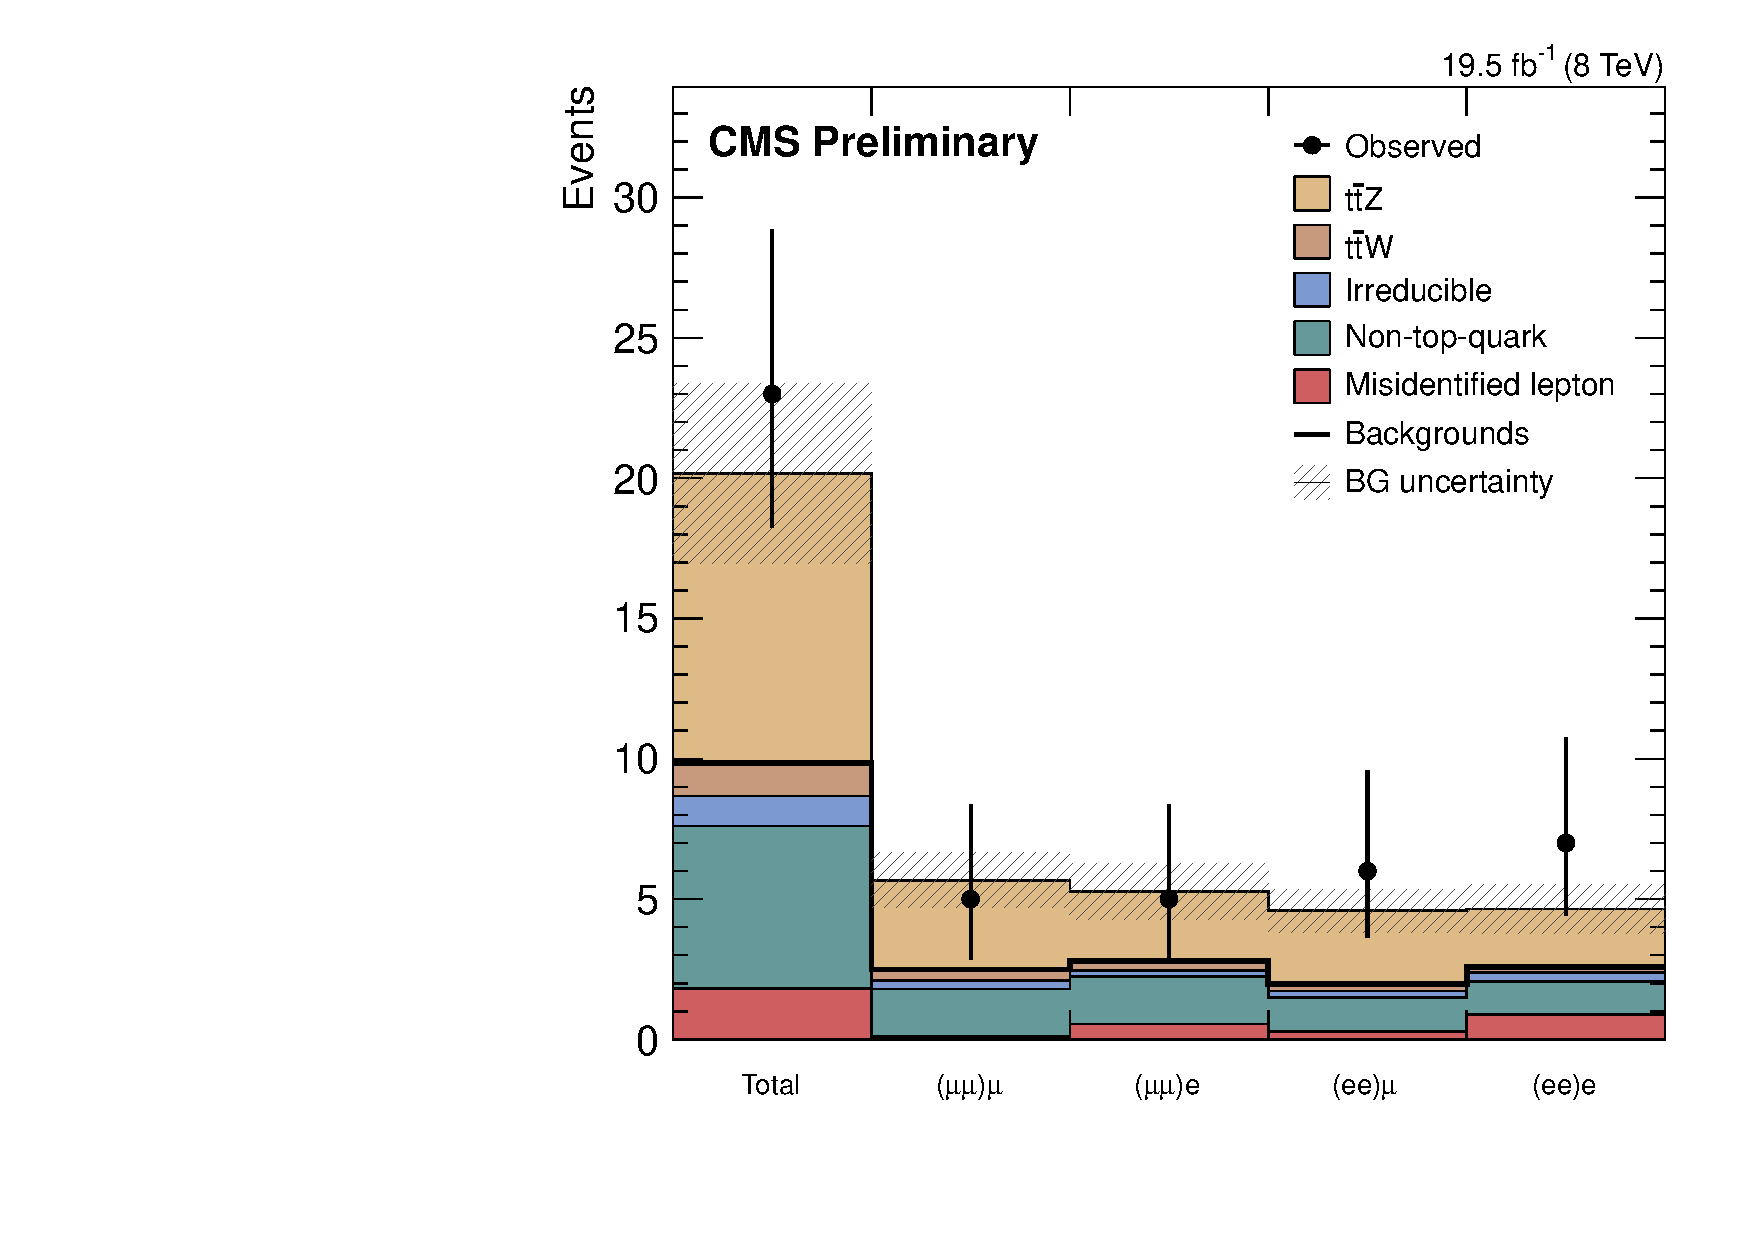
\includegraphics[width=0.48\linewidth]{Figs/Plots_PreSelections/hYields_3L2b.pdf}
\caption{\label{fig:hyields_3L2b}
Yields with break down by leptonic channel of data and predictions after tri-lepton plus two b-tag selections.
}
\end{center}
\end{figure}

\begin{figure}[h]
\begin{center}
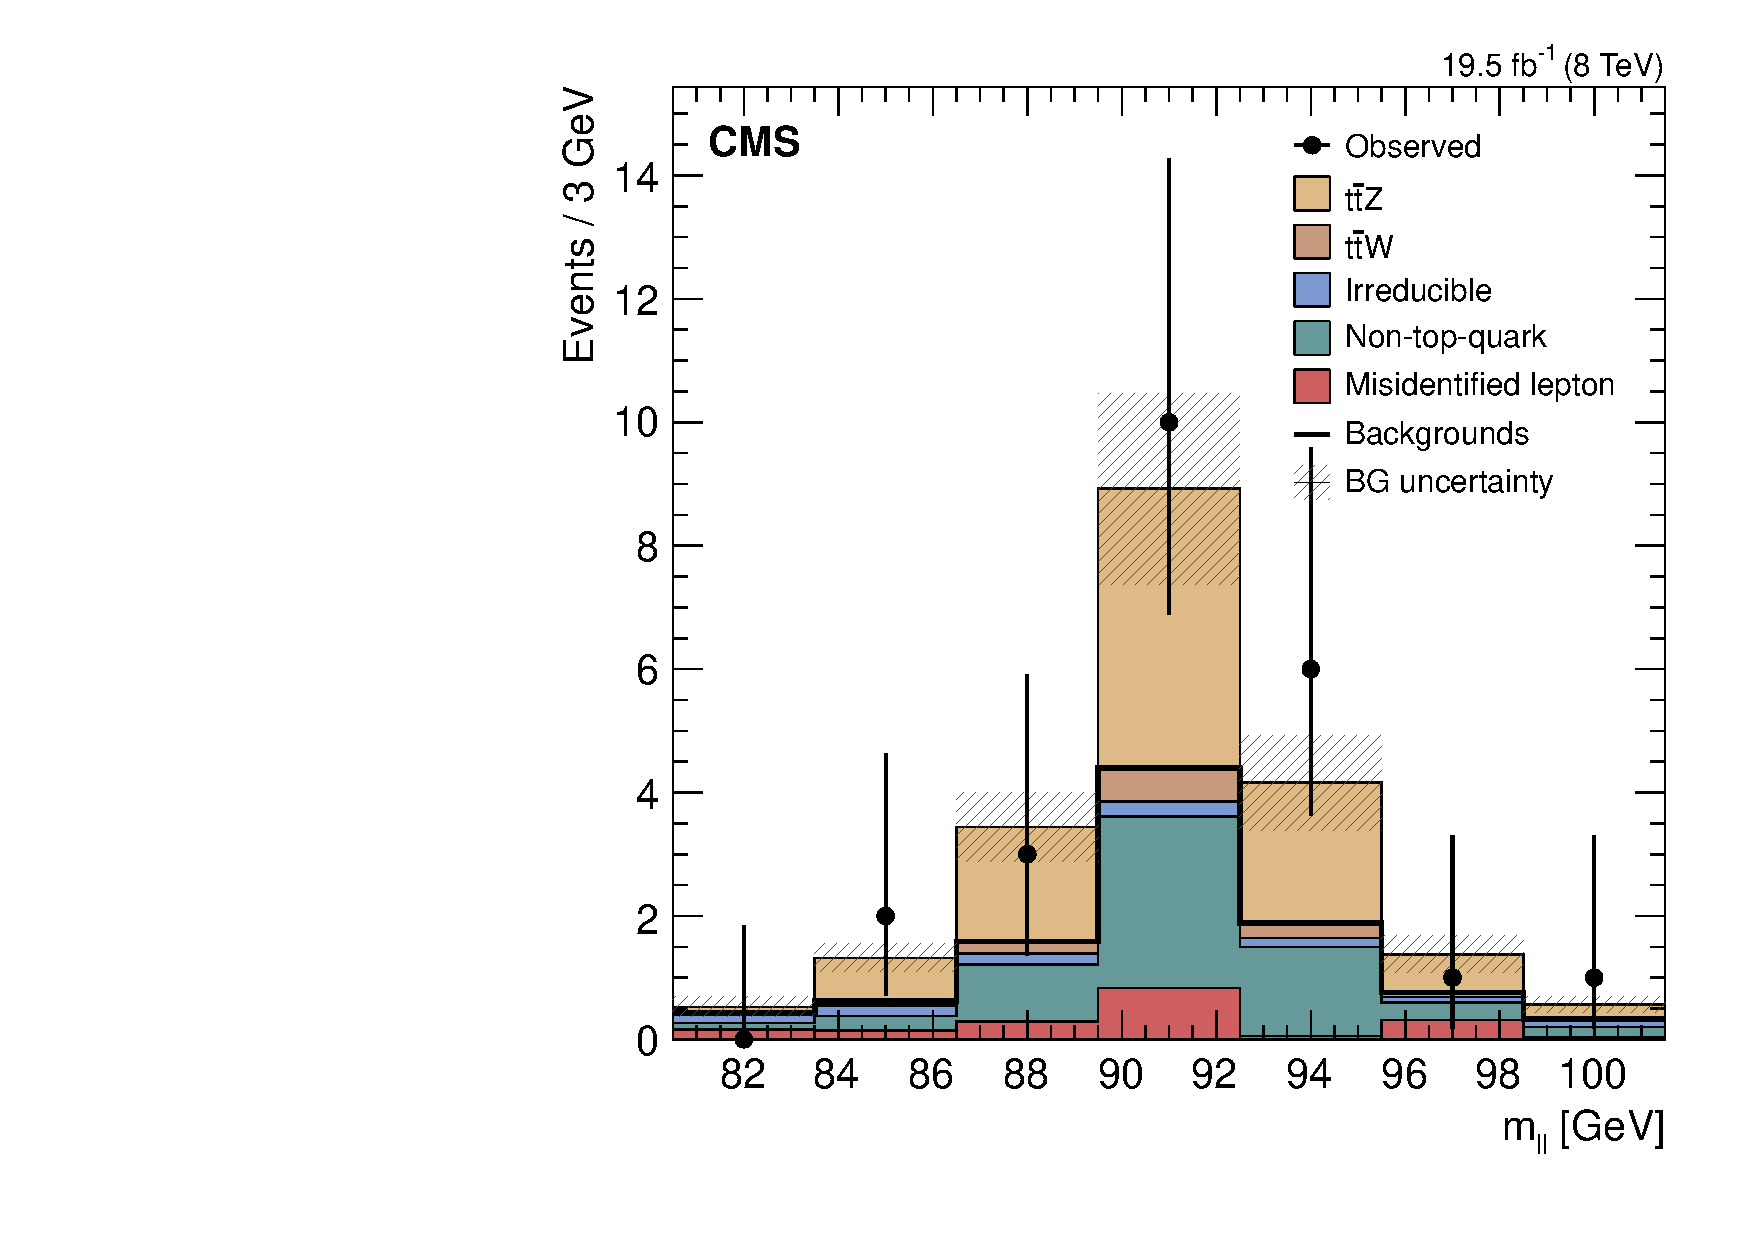
\includegraphics[width=0.48\linewidth]{Figs/Plots_PreSelections/hZMass_3L2b.pdf}
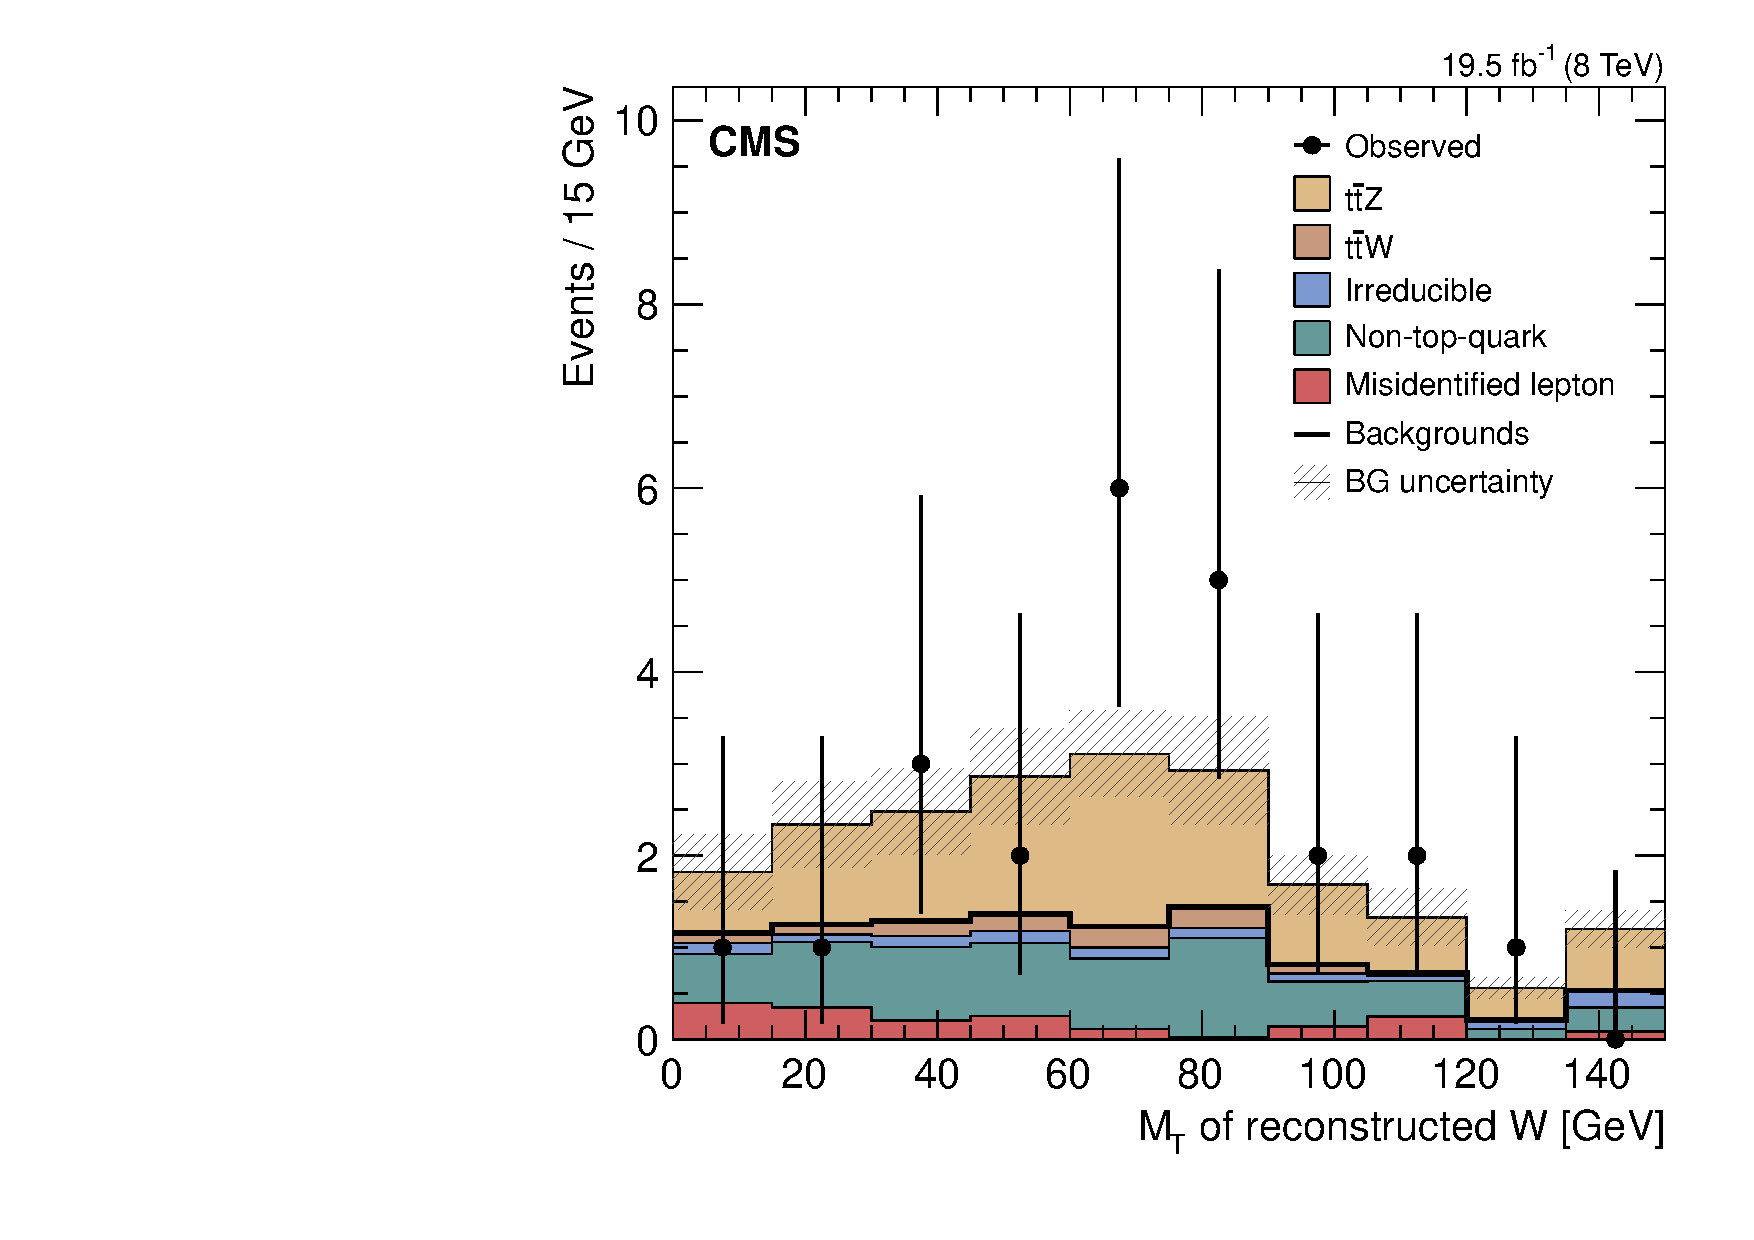
\includegraphics[width=0.48\linewidth]{Figs/Plots_PreSelections/hWMt_3L2b.pdf}
\caption{\label{fig:hmass_3L2b}
Reconstructed mass plots after tri-lepton plus two b-tag selections. Reconstructed Z Mass from lepton pair (Left). Reconstructed W \Mt \ (Right ).
}
\end{center}
\end{figure}


\begin{figure}[h]
\begin{center}
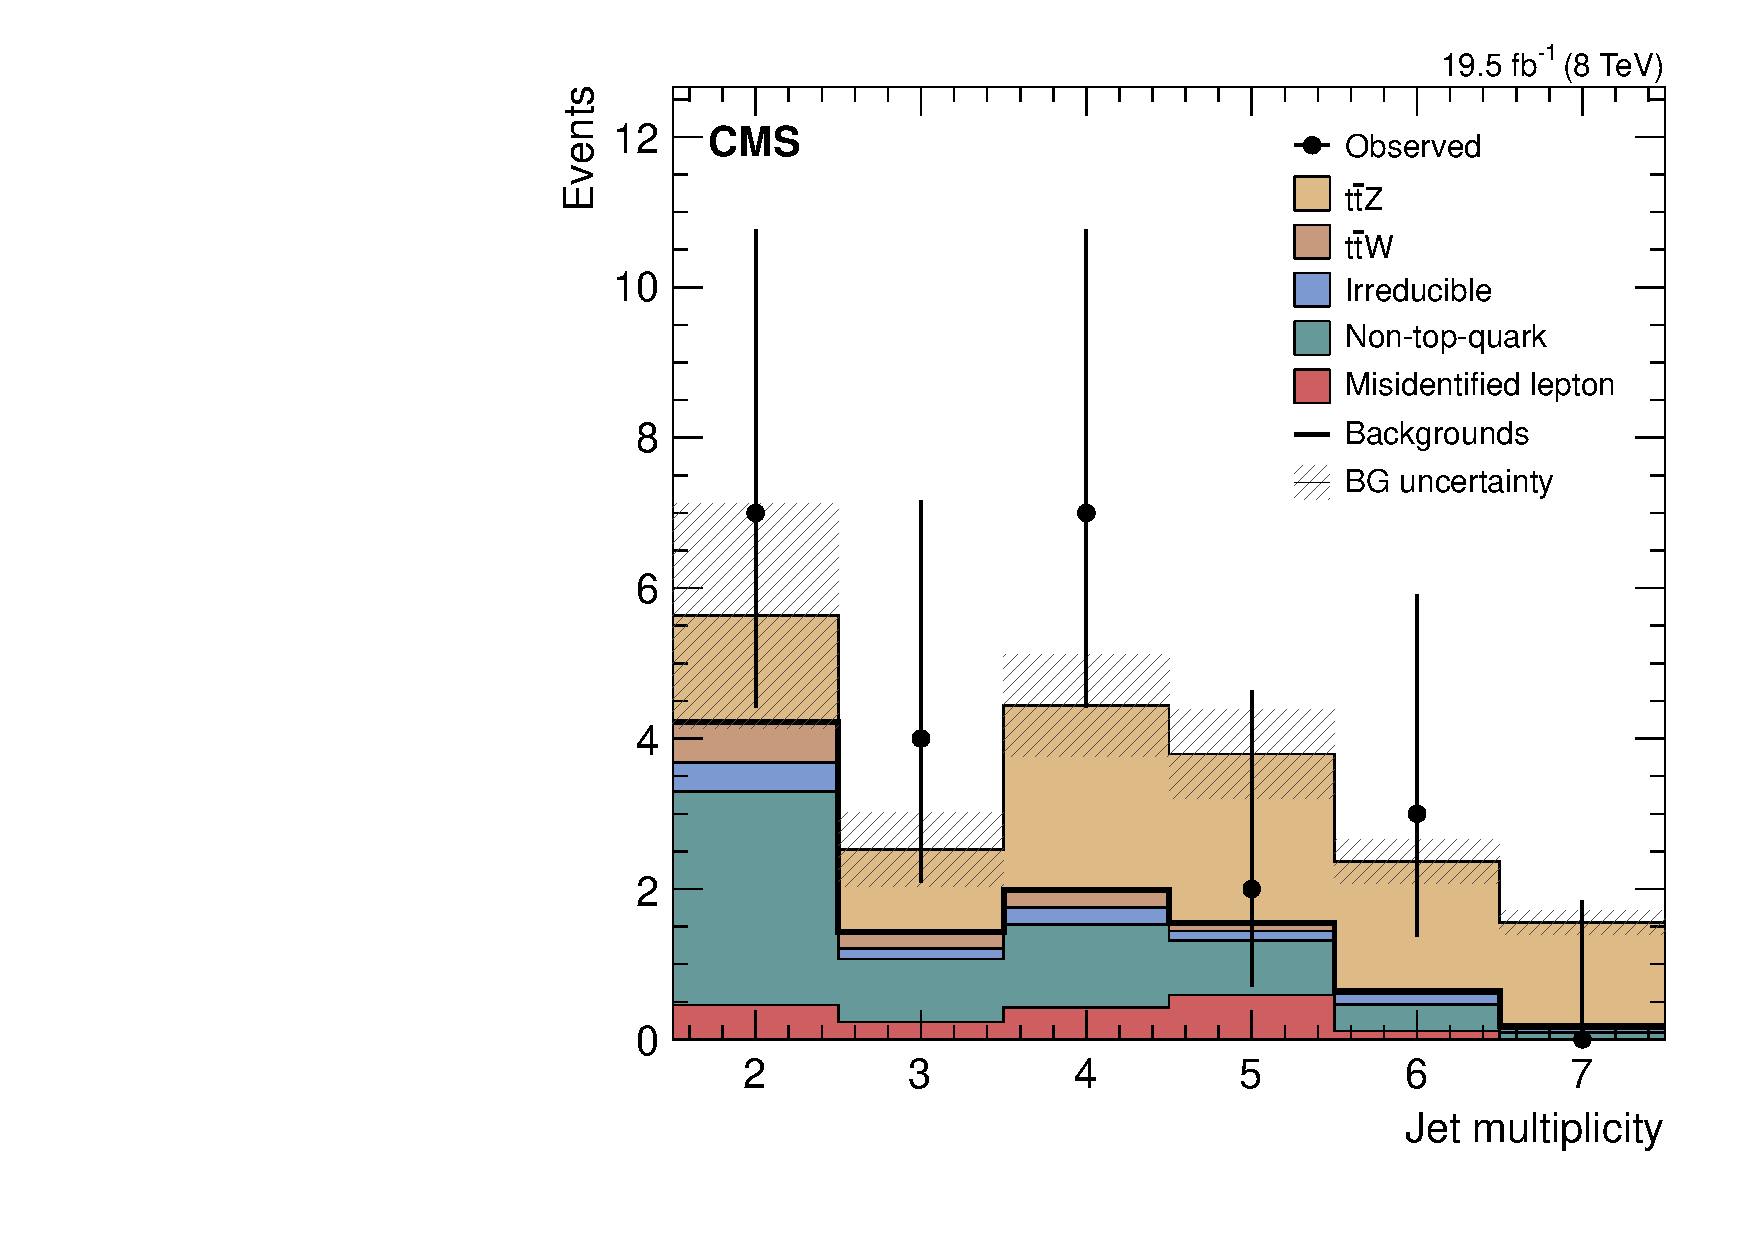
\includegraphics[width=0.48\linewidth]{Figs/Plots_PreSelections/hNJets_3L2b.pdf}
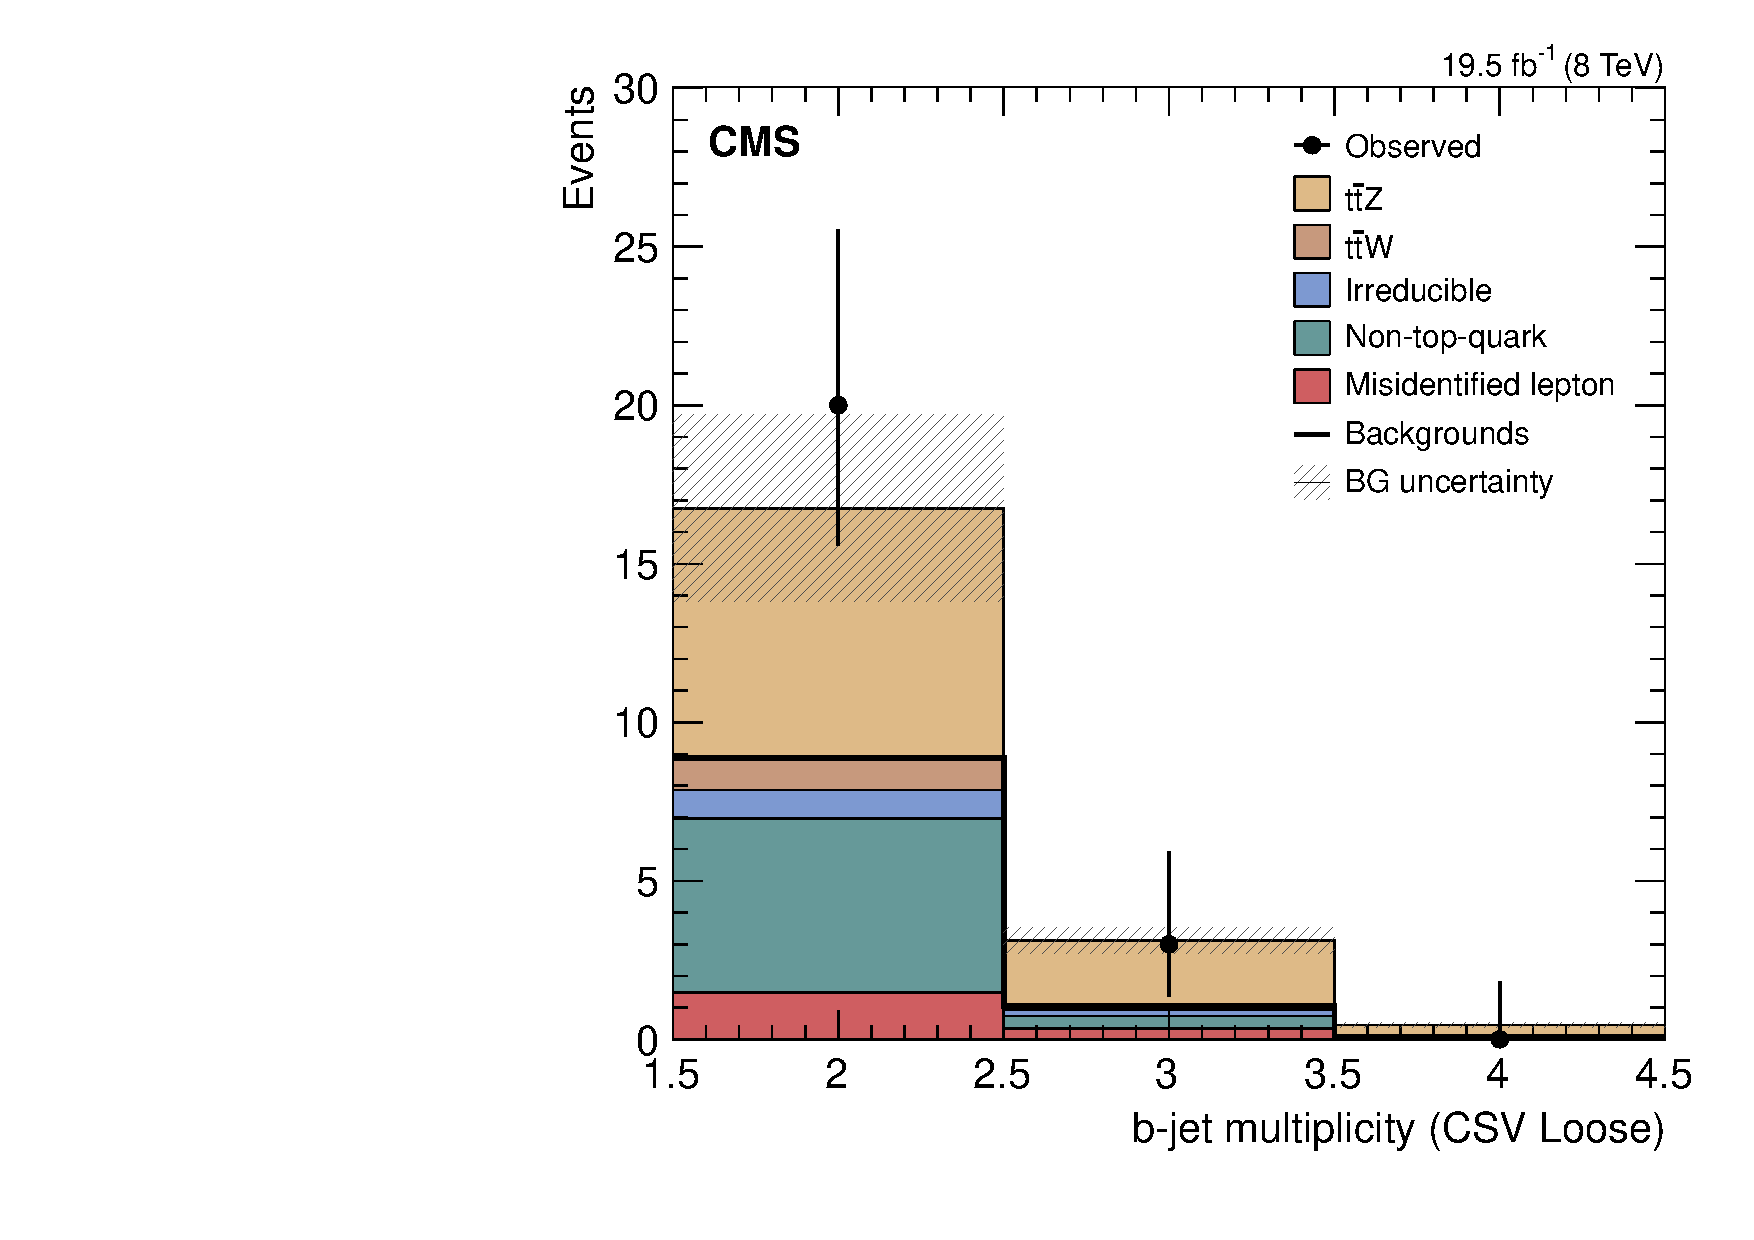
\includegraphics[width=0.48\linewidth]{Figs/Plots_PreSelections/hNLoose_3L2b.pdf}
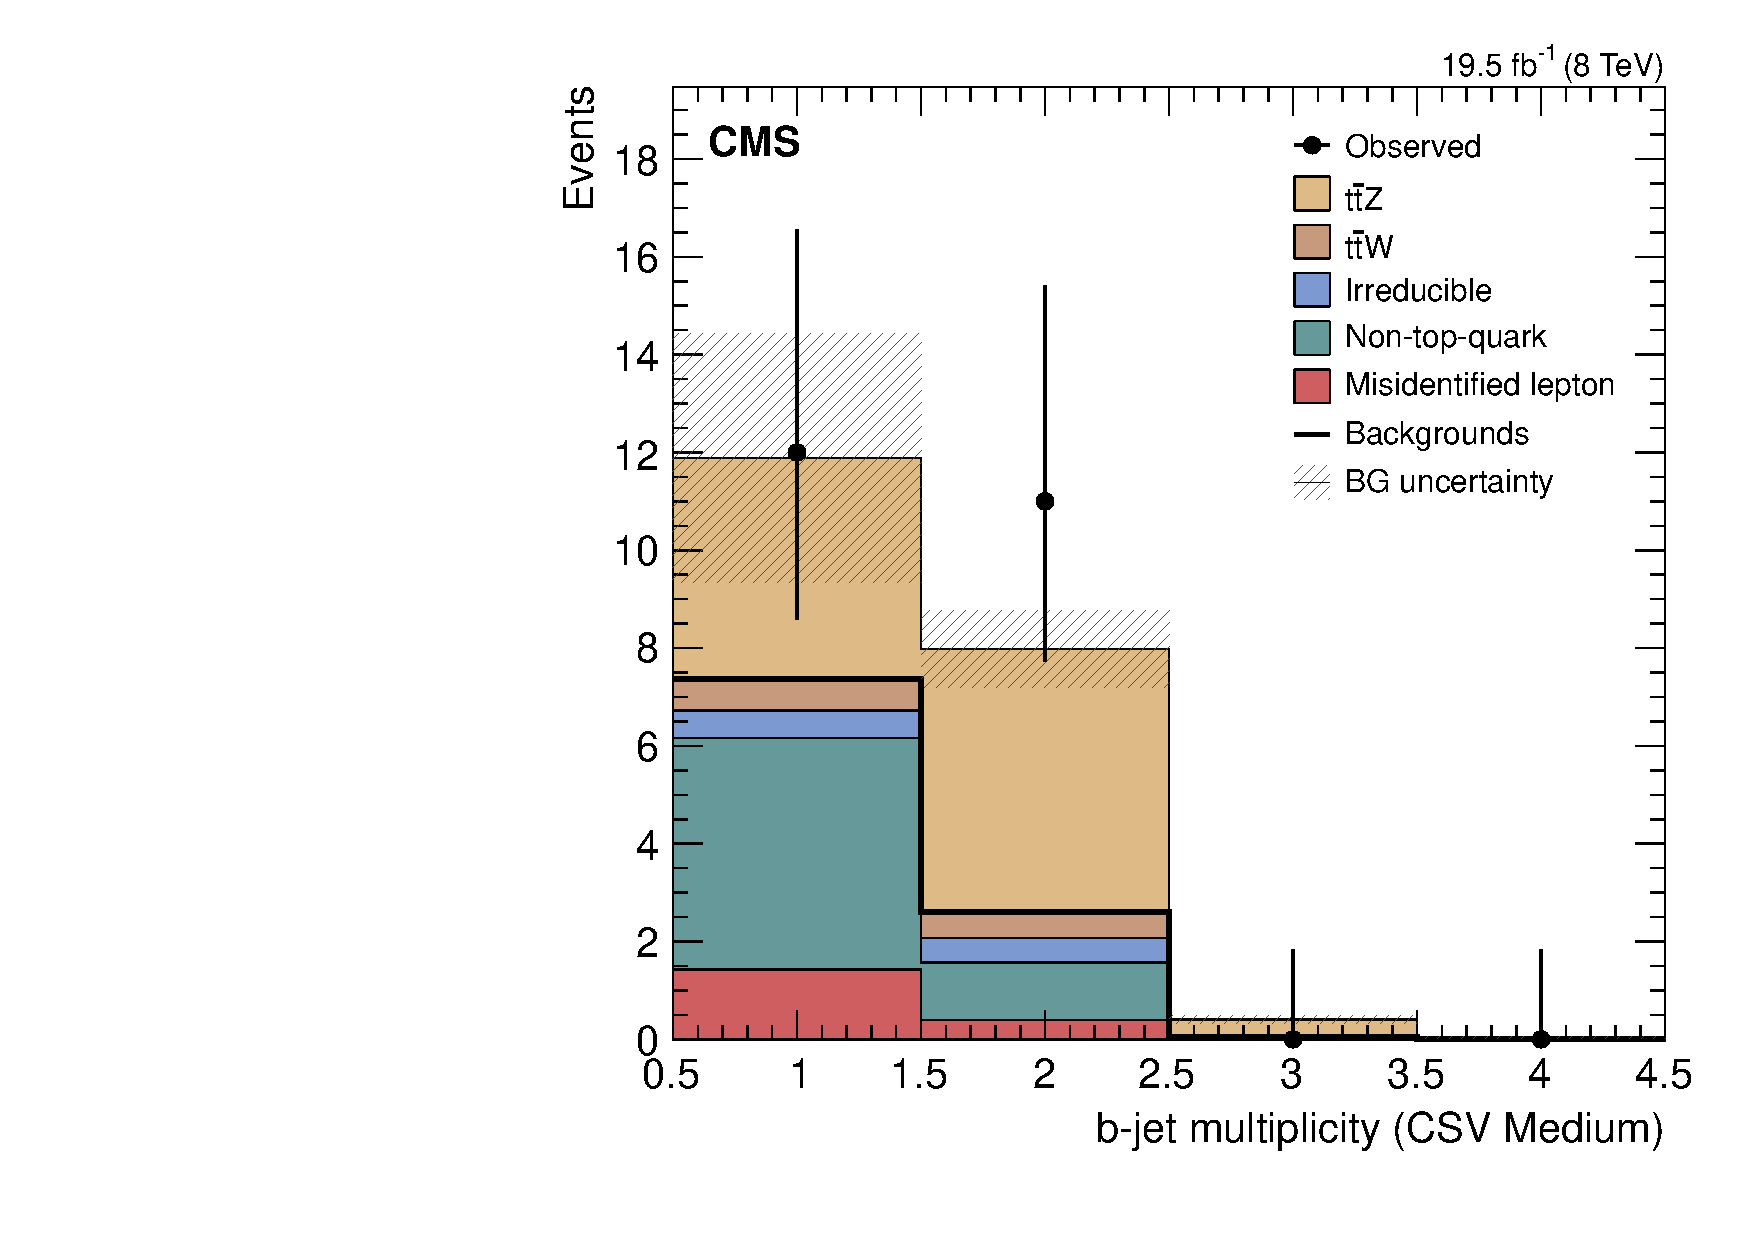
\includegraphics[width=0.48\linewidth]{Figs/Plots_PreSelections/hNMedium_3L2b.pdf}
\caption{\label{fig:jetmult_3L2b}
Jet Multiplicities. Left: Number of pfJets after tri-lepton plus two b-tag selections. Middle: Number of CSVL b-tags. Right: Number of CSVM b-tags.
}
\end{center}
\end{figure}


\begin{figure}[h]
\begin{center}
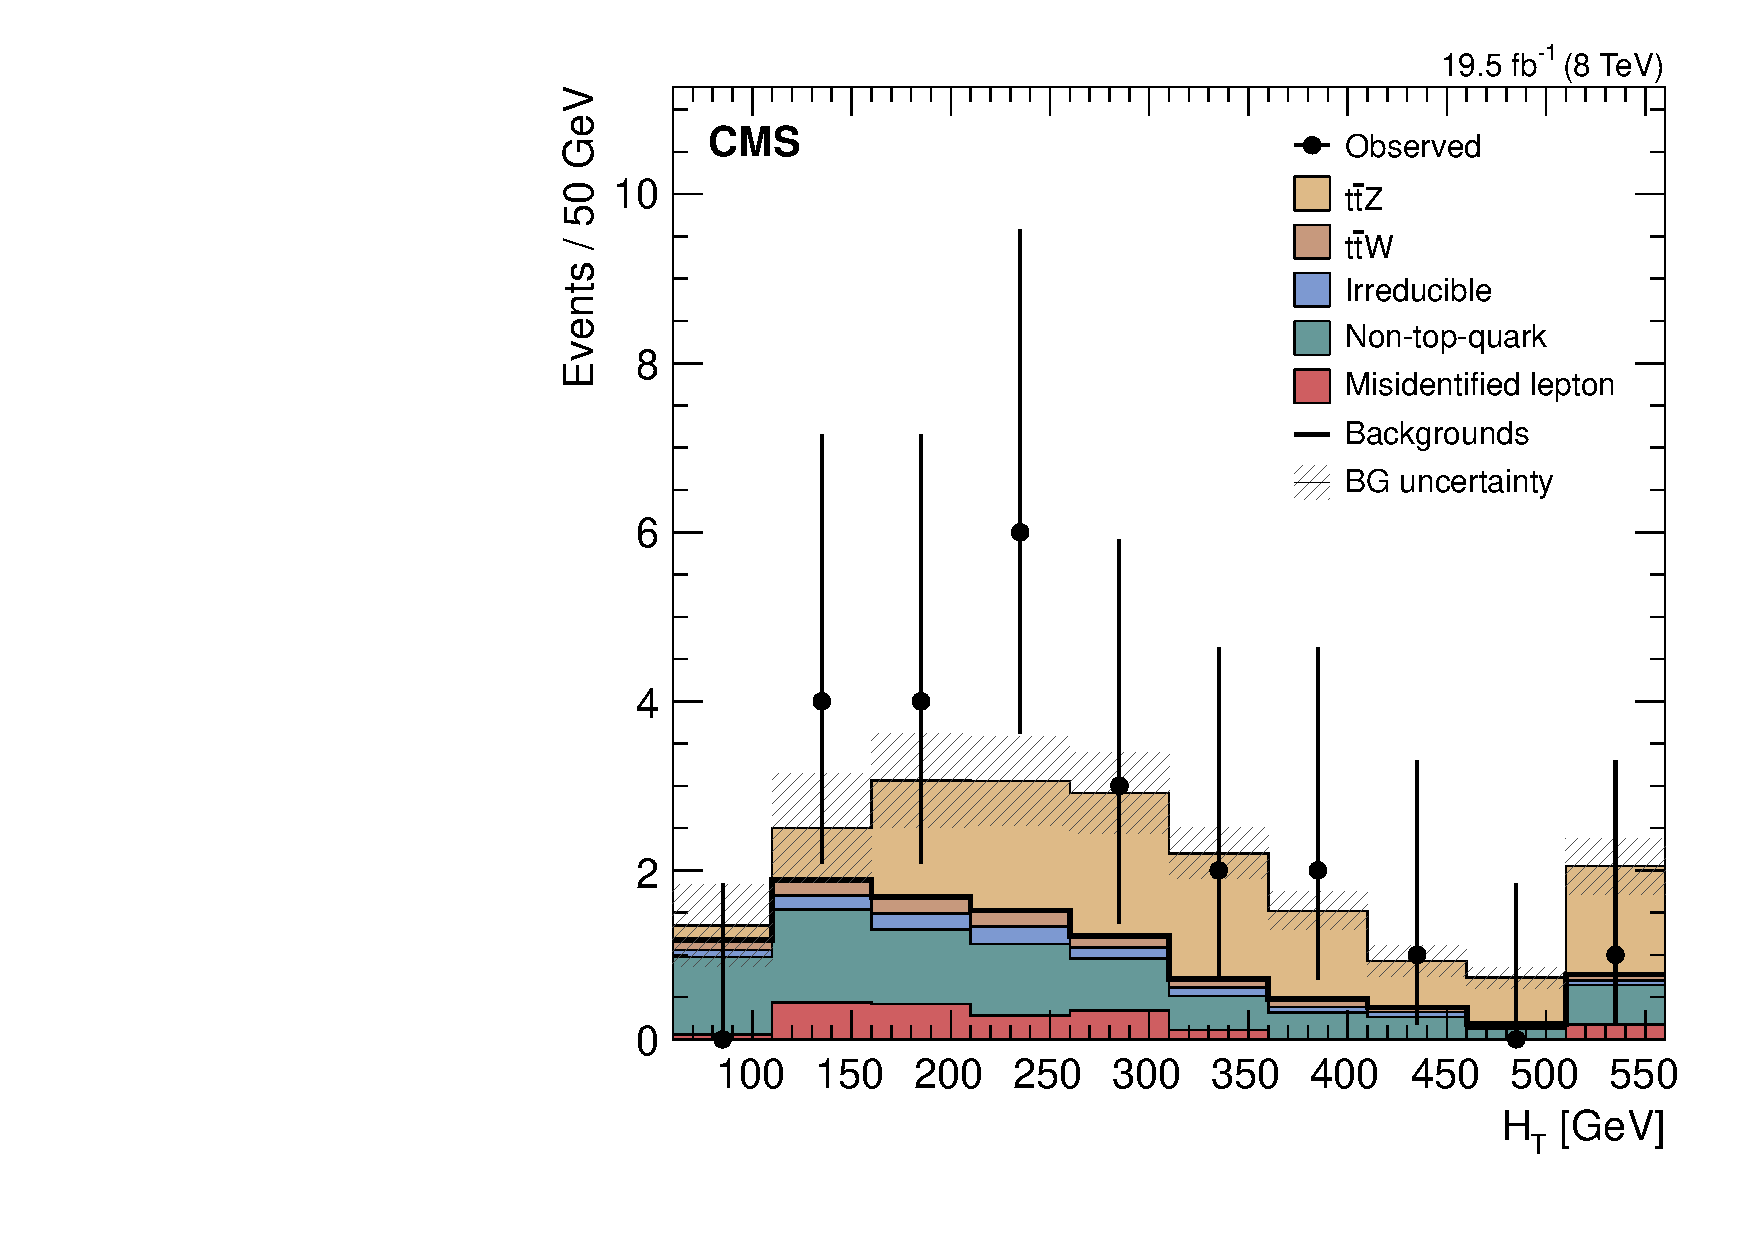
\includegraphics[width=0.48\linewidth]{Figs/Plots_PreSelections/hHt_3L2b.pdf}
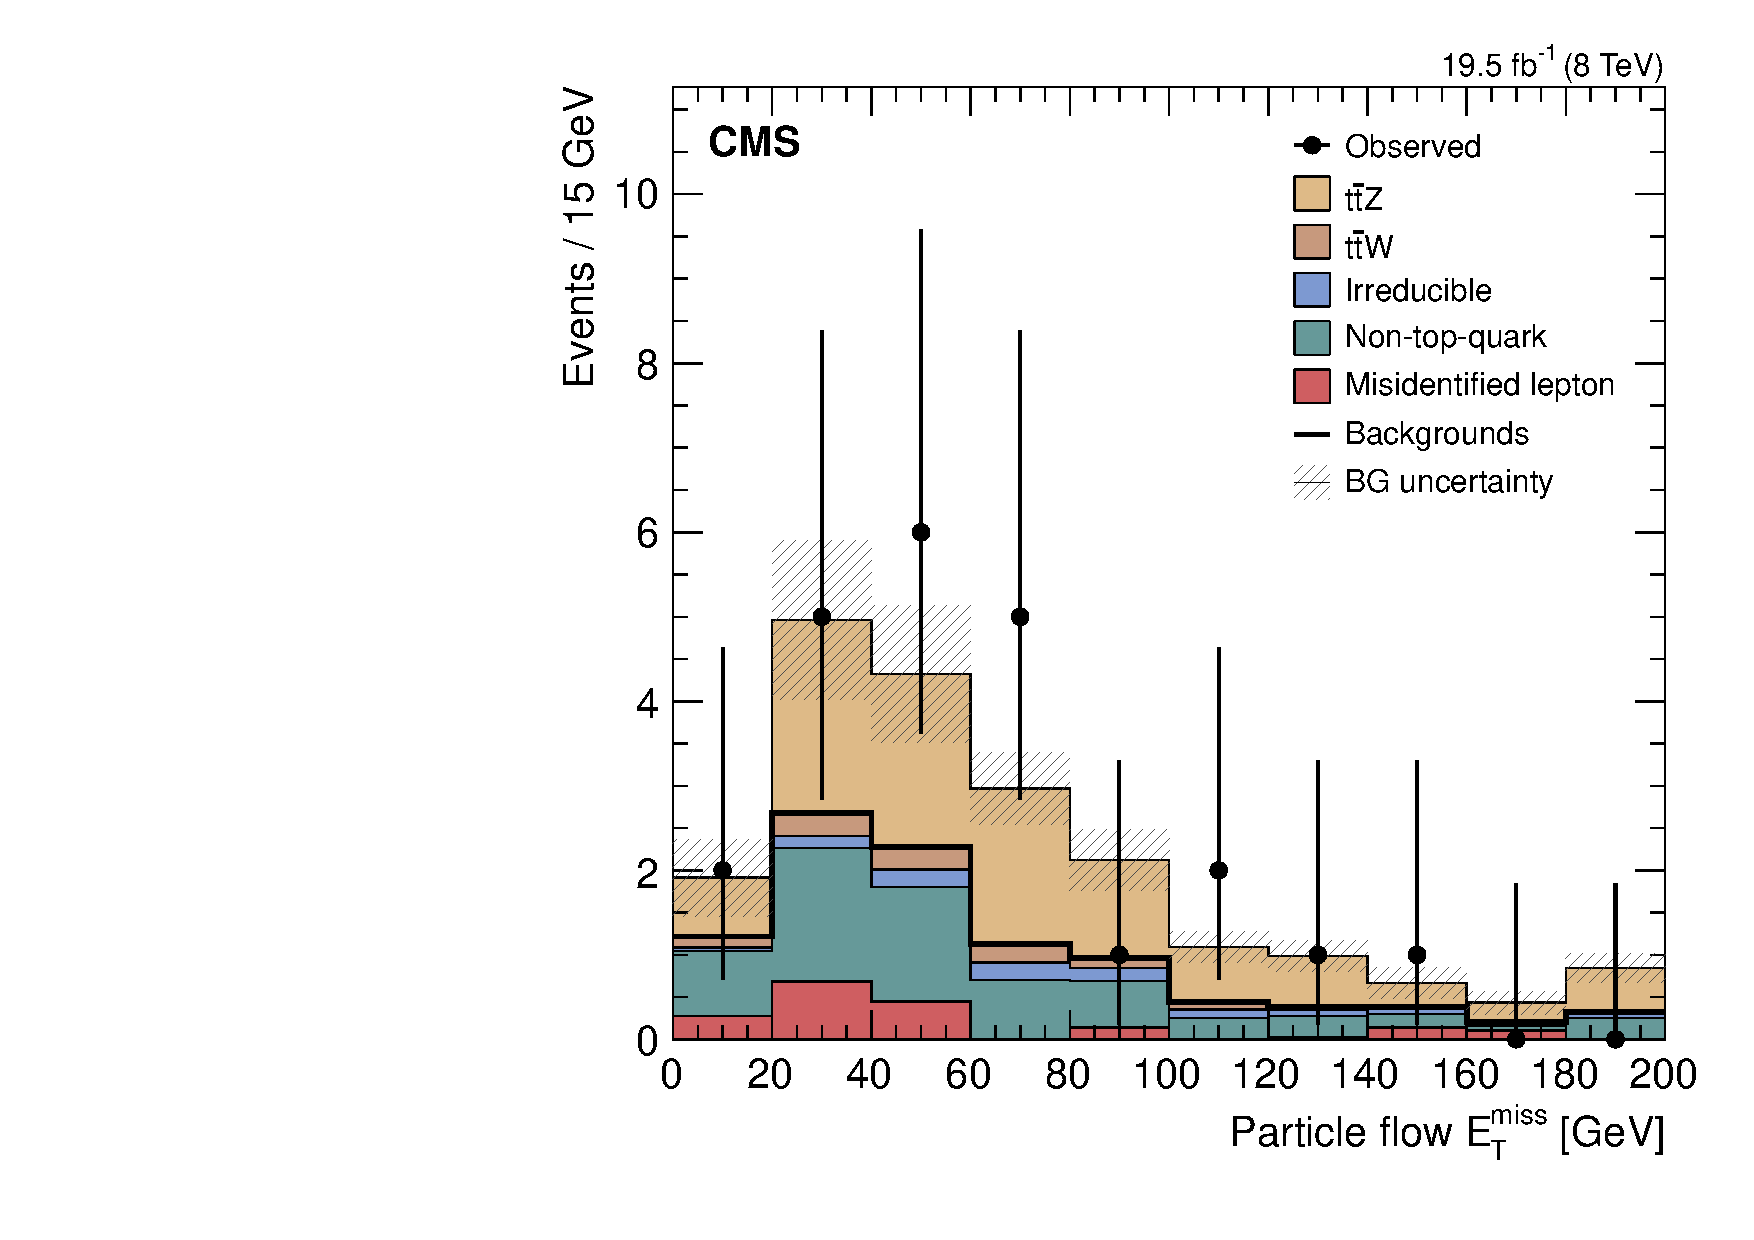
\includegraphics[width=0.48\linewidth]{Figs/Plots_PreSelections/hPFMet_3L2b.pdf}
\caption{\label{fig:hht_pfmet_3l}
Ht (Left) and pfMet (Right) after tri-lepton plus two b-tag selections.
}
\end{center}
\end{figure}







         
	\section{Yields from Data After Full Selections}
	The yields in data and MC are summarized in Table~\ref{tab:yields} after applying the full analysis selections as listed in Sec~\ref{sec:EventSelections}. The MC is normalized to \intLumi of luminosity to match the data, and scaled by the lepton efficiency scale factors and b-tag discriminant re-weighting as described in Sections~\ref{sec:tag_and_probe} and~\ref{sec:btag_syst} respectively. The data yields are shown along side the MC yields to help demonstrate the relative contributions of the individual backgrounds. The data driven backgrounds were shown in a previous section and will be used in the next section to calculate the \ttZ \ signal. The irreducible backgrounds will be estimated from the yields in Table~\ref{tab:yields} using the line labeled $t\overline{t}$X/tbZ/VZZ. Given our lack of knowledge of cross sections for these processes and an inability to validate these MC samples against data, we assign a 50\% systematic.

\begin{sidewaystable}[ht!]
\begin{center}

\begin{tabular}{c|ccccc}\hline
&Yields (All)&Yields ($\mu\mu\mu$)&Yields ($\mu\mu$e)&Yields (ee$\mu$)&Yields (eee)\\
\hline \hline
W $\rightarrow \ell \nu$ & 0.00$\pm$0.89 & 0.00$\pm$0.89 & 0.00$\pm$0.89 & 0.00$\pm$0.89 & 0.00$\pm$0.89\\
VV $\rightarrow 2 \ell$ & 0.04$\pm$0.07 & 0.02$\pm$0.06 & 0.02$\pm$0.06 & 0.00$\pm$0.06 & 0.00$\pm$0.06\\
$t\overline{t}$ & 0.32$\pm$0.12 & 0.11$\pm$0.08 & 0.14$\pm$0.10 & 0.04$\pm$0.09 & 0.03$\pm$0.09\\
DY $\rightarrow 2 \ell$  & 0.00$\pm$0.60 & 0.00$\pm$0.60 & 0.00$\pm$0.60 & 0.00$\pm$0.60 & 0.00$\pm$0.60\\
VZ $\rightarrow 3\ell$ or $4\ell$ & 1.02$\pm$0.09 & 0.25$\pm$0.04 & 0.34$\pm$0.05 & 0.19$\pm$0.04 & 0.23$\pm$0.04\\
WWV & 0.13$\pm$0.03 & 0.03$\pm$0.01 & 0.02$\pm$0.01 & 0.05$\pm$0.02 & 0.03$\pm$0.01\\
\ttX/tbZ/VZZ & 0.98$\pm$0.08 & 0.32$\pm$0.05 & 0.20$\pm$0.04 & 0.24$\pm$0.05 & 0.22$\pm$0.04\\
\ttZ & 8.15$\pm$0.38 & 2.45$\pm$0.21 & 2.09$\pm$0.19 & 1.99$\pm$0.19 & 1.62$\pm$0.17\\
\hline \hline
Total Bkg MC (19.5 fb$^{-1}$) & 2.49$\pm$1.09 & 0.74$\pm$1.08 & 0.72$\pm$1.08 & 0.51$\pm$1.08 & 0.52$\pm$1.08\\
\hline
Total Sig+Bkg MC (19.5 fb$^{-1}$) & 10.64$\pm$1.15 & 3.19$\pm$1.10 & 2.81$\pm$1.10 & 2.50$\pm$1.10 & 2.14$\pm$1.09\\
\hline
Data (19.5 fb$^{-1}$) & 12.$\pm$3.46 & 3.$\pm$1.73 & 2.$\pm$1.41 & 4.$\pm$2.00 & 3.$\pm$1.73\\
\hline
\end{tabular}
\caption{ \label{tab:yields} Data and pure MC yields after full analysis selections with \intLumi.}
\end{center}
\end{sidewaystable}

\clearpage

	\section{Measured Signal and Background Subtraction}
	\label{sec:signal}
Compiling the information in the preceding sections, an estimate can be made for the \ttZ \ signal in the measured data. The contribution due to di-lepton final states that pass the selection due to an additional ``fake" lepton in the event is described in Sec~\ref{sec:fake_estimation} and the contribution from tri-lepton events that pass the selection due to b-tagged jets that arise from gluon radiation is described in Sec~\ref{sec:brate_estimation}. Finally, the irreducible backgrounds which cannot be estimated by a data driven method are taken from the row labeled ``\ttX/tbZ/VZZ" in Table~\ref{tab:yields} where the ``X" is short hand for W, $\gamma$, or WW. Table~\ref{tab:signal_minus_bkg} summarizes the full yields in data after selections as well as the background estimates. Additionally a final estimate for the \ttZ \ to three lepton signal is shown.

\begin{table}[ht!]
\begin{center}

\begin{tabular}{c|c}\hline
 & Measurement\\
\hline \hline
Data (19.5 fb $^{-1}$)                         & $12. $ \\
%\hdashline
Bkg from Non-Prompt Leptons                   &  $- 1.13 \pm 0.51_{st} \pm 0.57_{sy}$ \\
Bkg from b-tags From Radiation                &  $- 2.27 \pm 0.51_{st} \pm 1.14_{sy}$ \\
Bkg from Irreducible                          &  $- 0.98 \pm 0.08_{st} \pm 0.49_{sy}$ \\
%\hdashline
Total Background Prediction                   &  $-4.38 \pm 0.73_{bkg st} \pm 1.37_{bkg sy}$ \\
\hline
Predicted Signal                              &  $7.62 \pm 3.46_{data st} \pm 0.73_{bkg st} \pm 1.37_{bkg sy}$ \\	
\hline
\end{tabular}
\caption{ \label{tab:signal_minus_bkg} Data and pure MC yields after full analysis selections with \intLumi.}
\end{center}
\end{table}



	
	\subsection{Method for Reconstructing a Top Mass}
	The selections chosen allow the identification of all of the constituent components of the top which decays to final state quarks. A good test for the accuracy and purity of the selection is to recreate a top mass. Determining which  particles actually came from the top is difficult. With more total events in the final selection to choose from, a more complicated but somewhat accurate algorithm could be chosen. With the lower number of events passing the selections in this document, a simple algorithm must be chosen to identify the jets from the hadronic top. There are few events, the algorithm must choose jets for each one, yet be simple enough not to sculpt the distribution. We following steps are taken:
\begin{enumerate}
\item Choose three jets, one of which has a CSVL or better b-tag that minimizes three jet system $\Delta R$ defined as
\begin{equation}
\Delta R_{j1,j2,b1} = \sqrt{ (\Delta R_{j1, ``top"}) ^2 + (\Delta R_{j2, ``top"}) ^2 + (\Delta R_{b1, ``top"}) ^2 }
\end{equation}
where ``top'' is the composite object created by summing the 4-vectors of the three jets.
\item Choose the highest pt b-jet out of the remaining b-tagged jets that are not part of the three jet system in step 1. This b-jet is considered to be from the leptonic top.
\end{enumerate}

Fig~\ref{fig:htopmass_3l2j2b} shows the hadronic top mass, hadronic W mass, and invariant mass of the b-jet and lepton from the leptonic top (with the neutrino unaccounted for for obvious reasons).


\begin{figure}[h]
\begin{center}
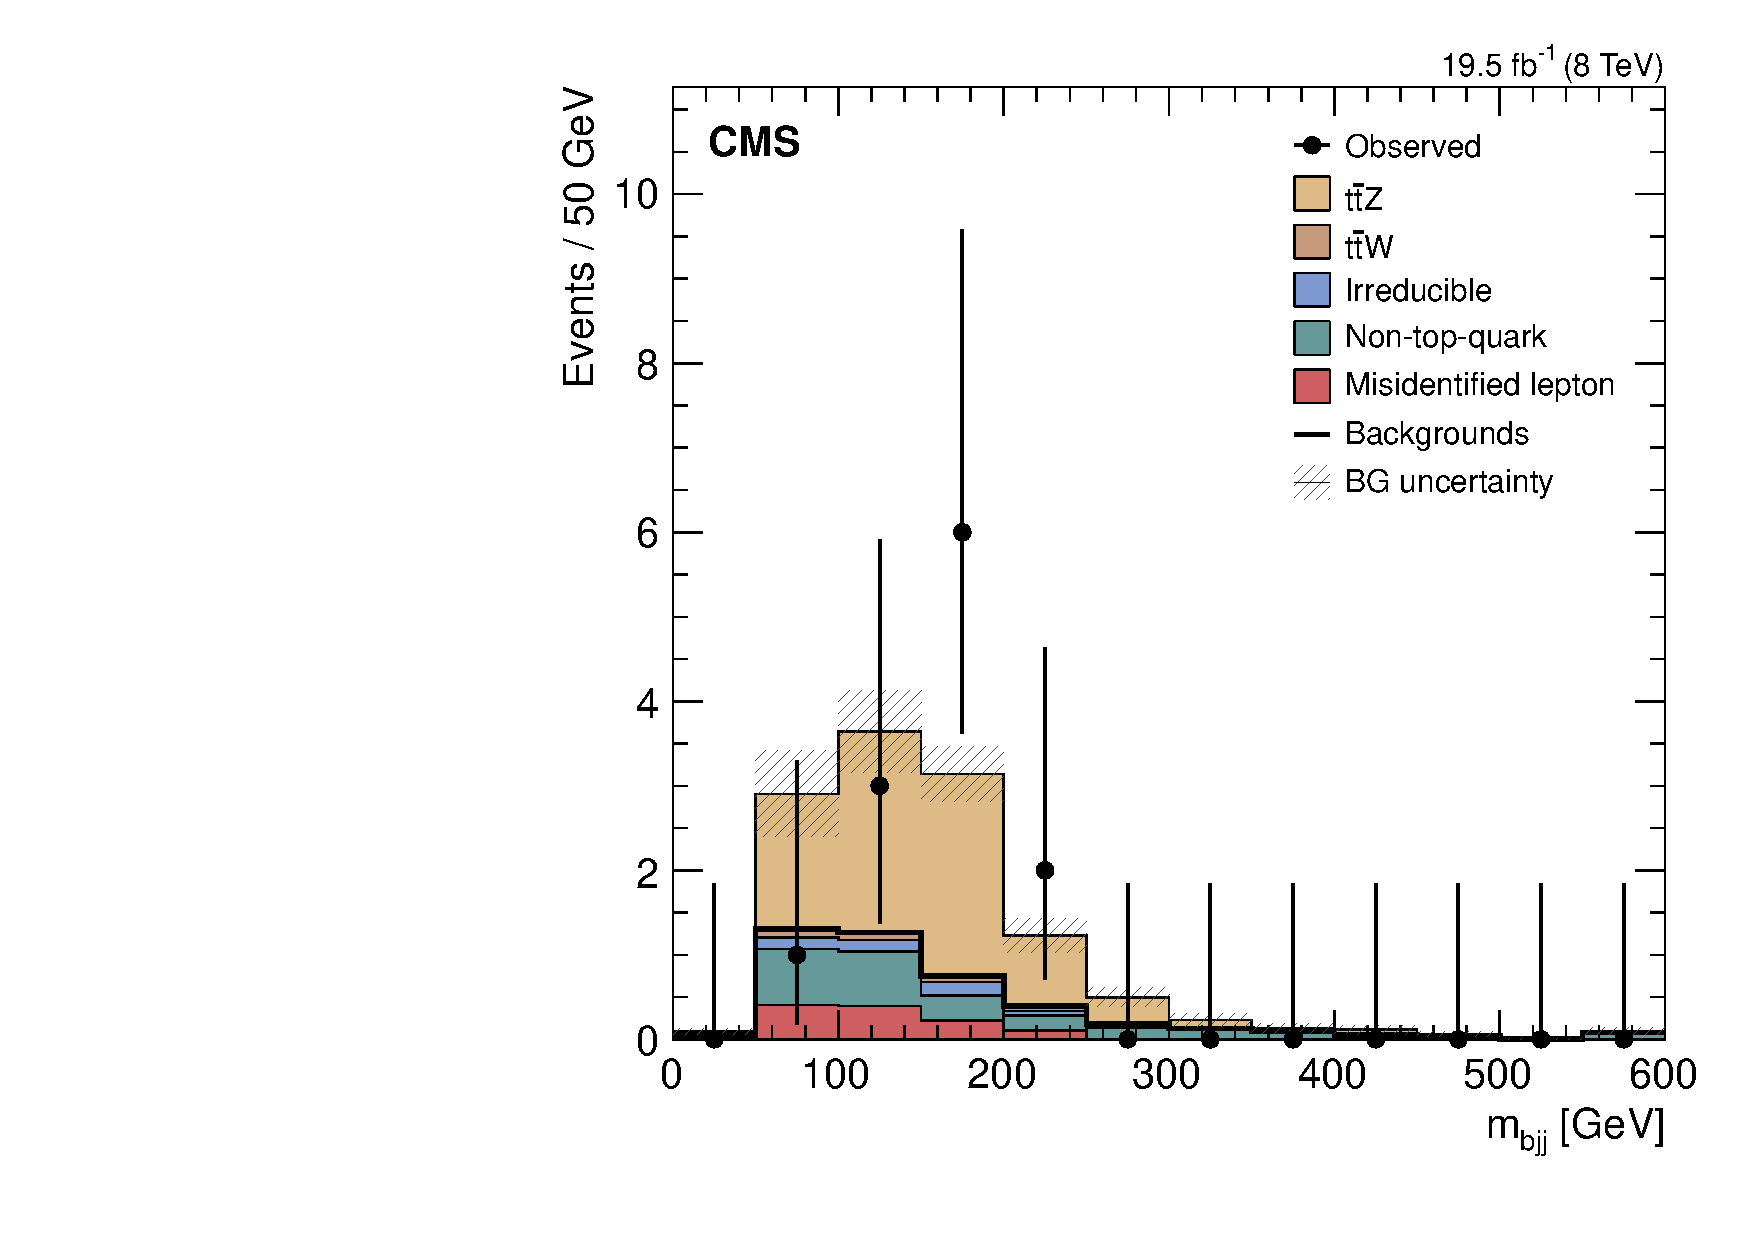
\includegraphics[width=0.48\linewidth]{Figs/Plots_Final_Selections/hTopMass_3L2J2b.pdf}
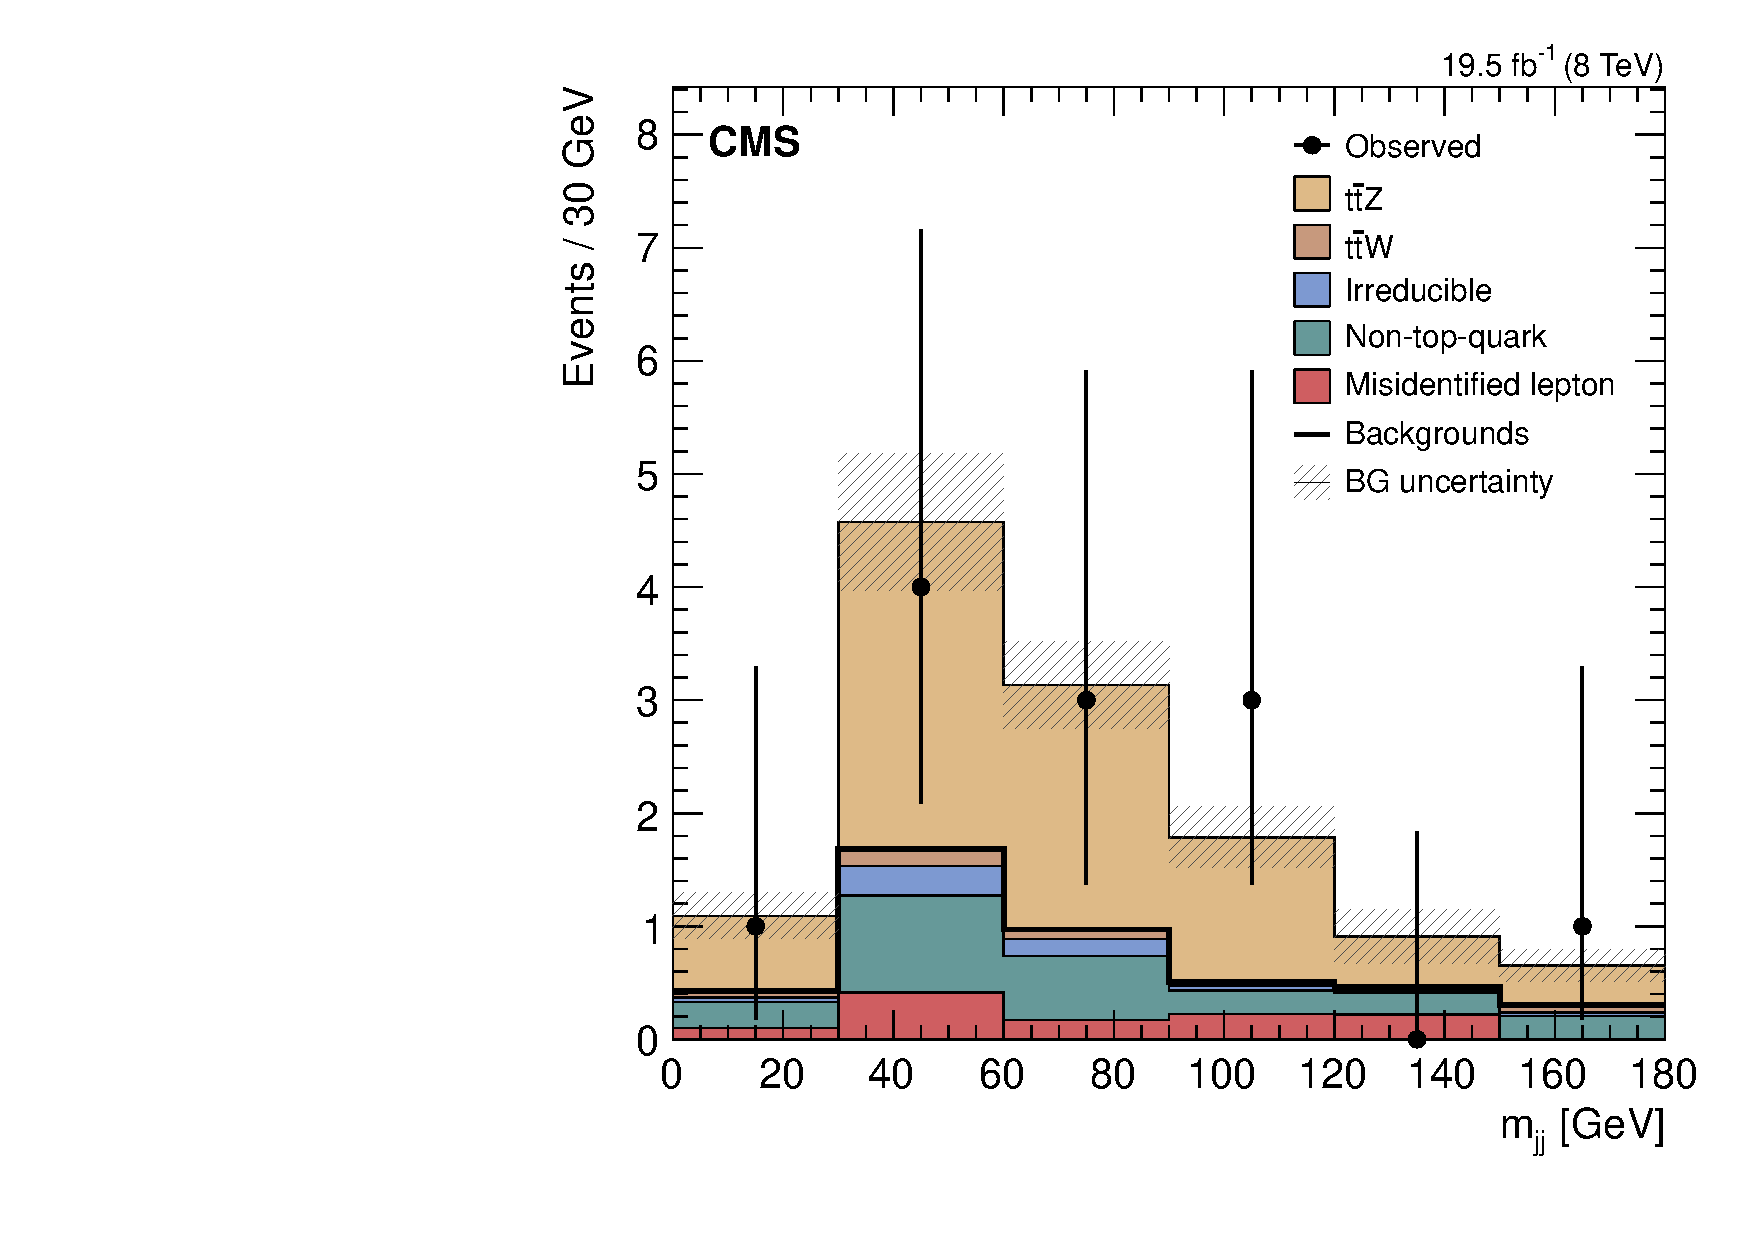
\includegraphics[width=0.48\linewidth]{Figs/Plots_Final_Selections/hTopWMass_3L2J2b.pdf}
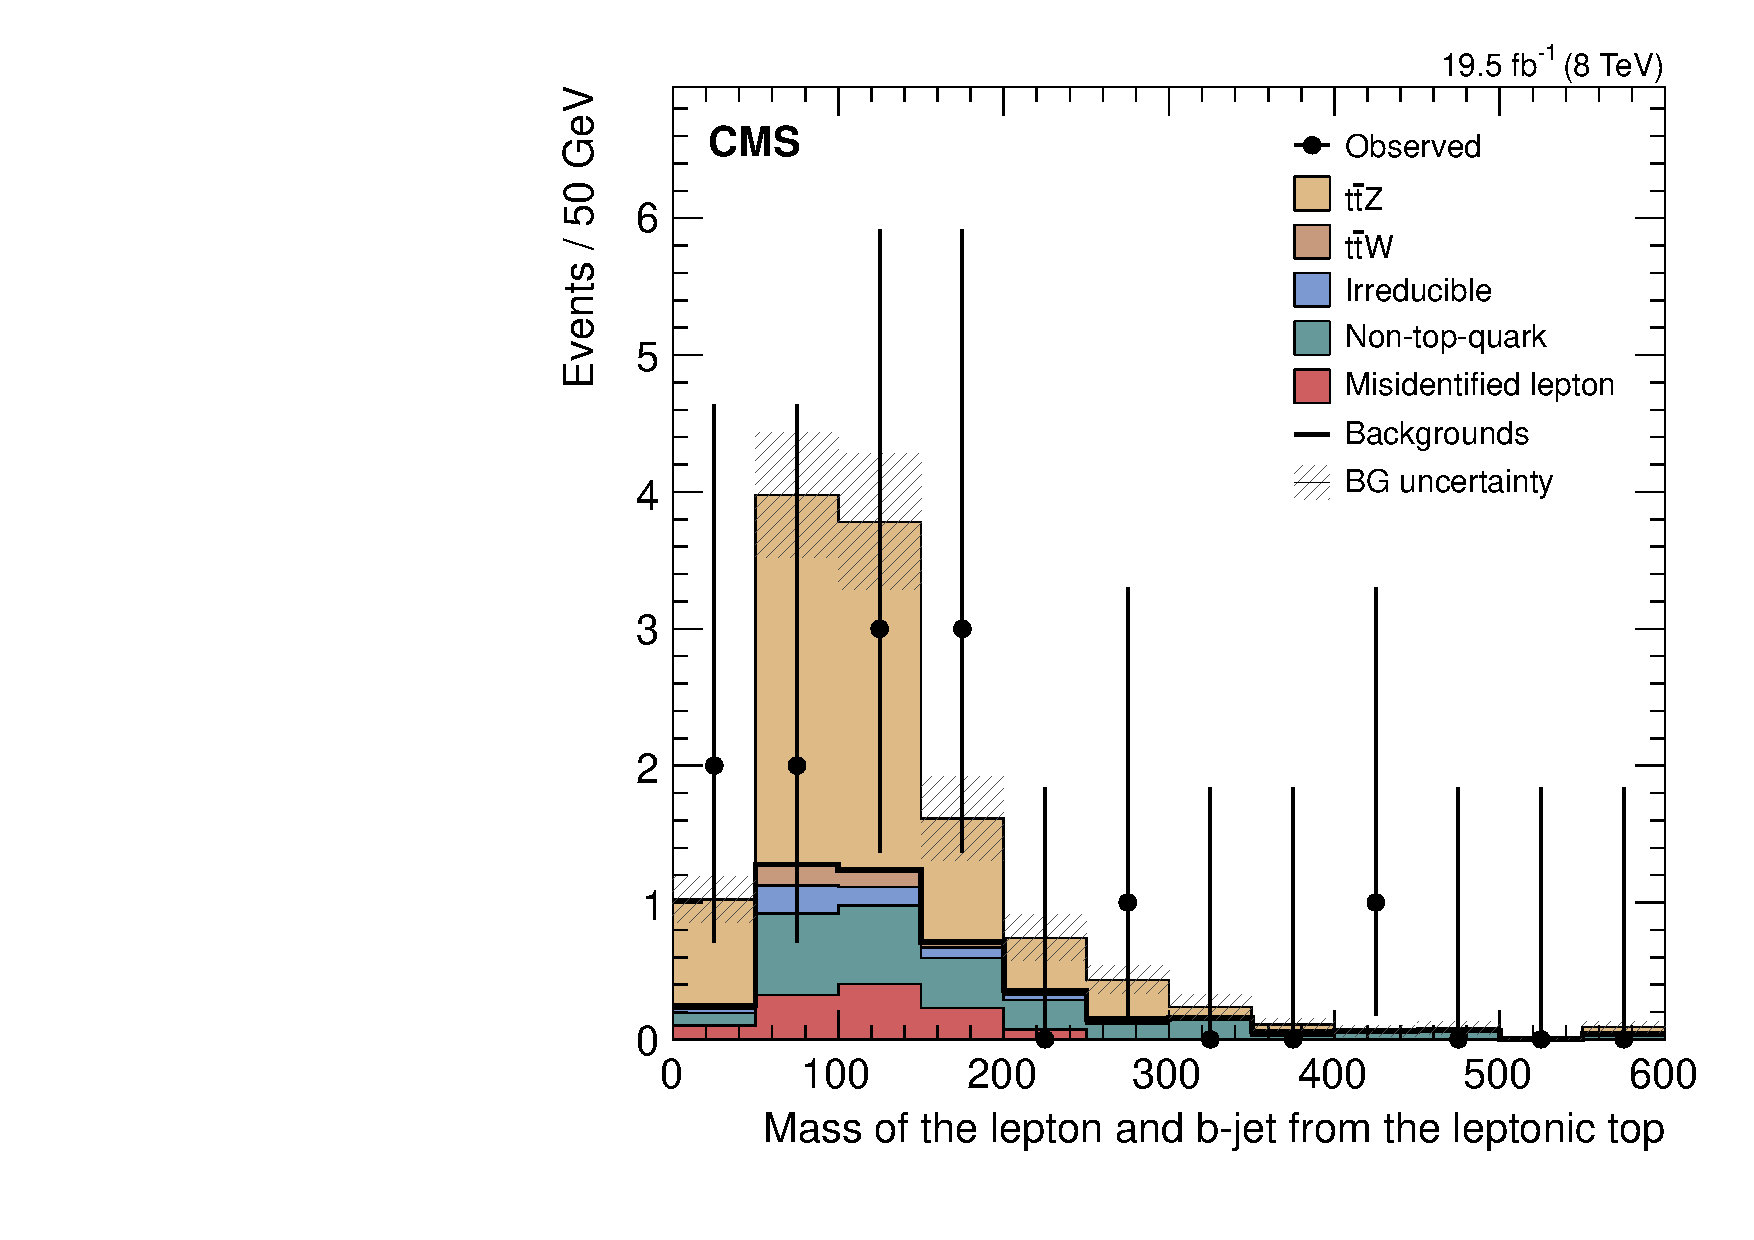
\includegraphics[width=0.48\linewidth]{Figs/Plots_Final_Selections/hTopbLMass_3L2J2b.pdf}
\caption{\label{fig:htopmass_3l2j2b}
Reconstructed mass of the hadronic top is shown after all selections have been applied (Top Left). Reconstructed mass of the hadronic W is shown after all selections have been applied(Top Right). Invariant mass of the W lepton with the b-jet from the leptonic top is shown (Bottom).
}
\end{center}
\end{figure}
	
	
	
	
	
	
	
	\subsection{Distributions with Full Selections}	
	
	The full analysis selection is described in Sec~\ref{sec:EventSelections}. This includes leptonic selections for reconstructing a Z from two leptons and requiring a third lepton that could be from a W. It also includes requiring four or more jets with two of them being b-tagged (one CSVL and one CSVM). After selection, the \ttZ \ contribution as predicted in MC is strong and the backgrounds have been reduced to a manageable level. In the following plots, data driven predictions are again used for normalization of backgrounds while MC is used for the shape (except in the case of the irreducible backgrounds where MC is used for shape and normalization). Although being lower in statistics, there is reasonable agreement between data and predictions (shape and size). Relevant plots are shown below. Fig~\ref{fig:hmass_3l2j2b} shows the reconstructed masses of the Z and the leptonic W (using \Mt) %while FIgure ~\ref{fig:htopmass_3l2j2b} shows the top (using the W \Mt \ for the W's contribution). 
These plots are used to demonstrate a degree of certainty that the correct events are being identified. %since the various underlying bosons and quarks can be reconstructed. \\

\begin{figure}[h]
\begin{center}
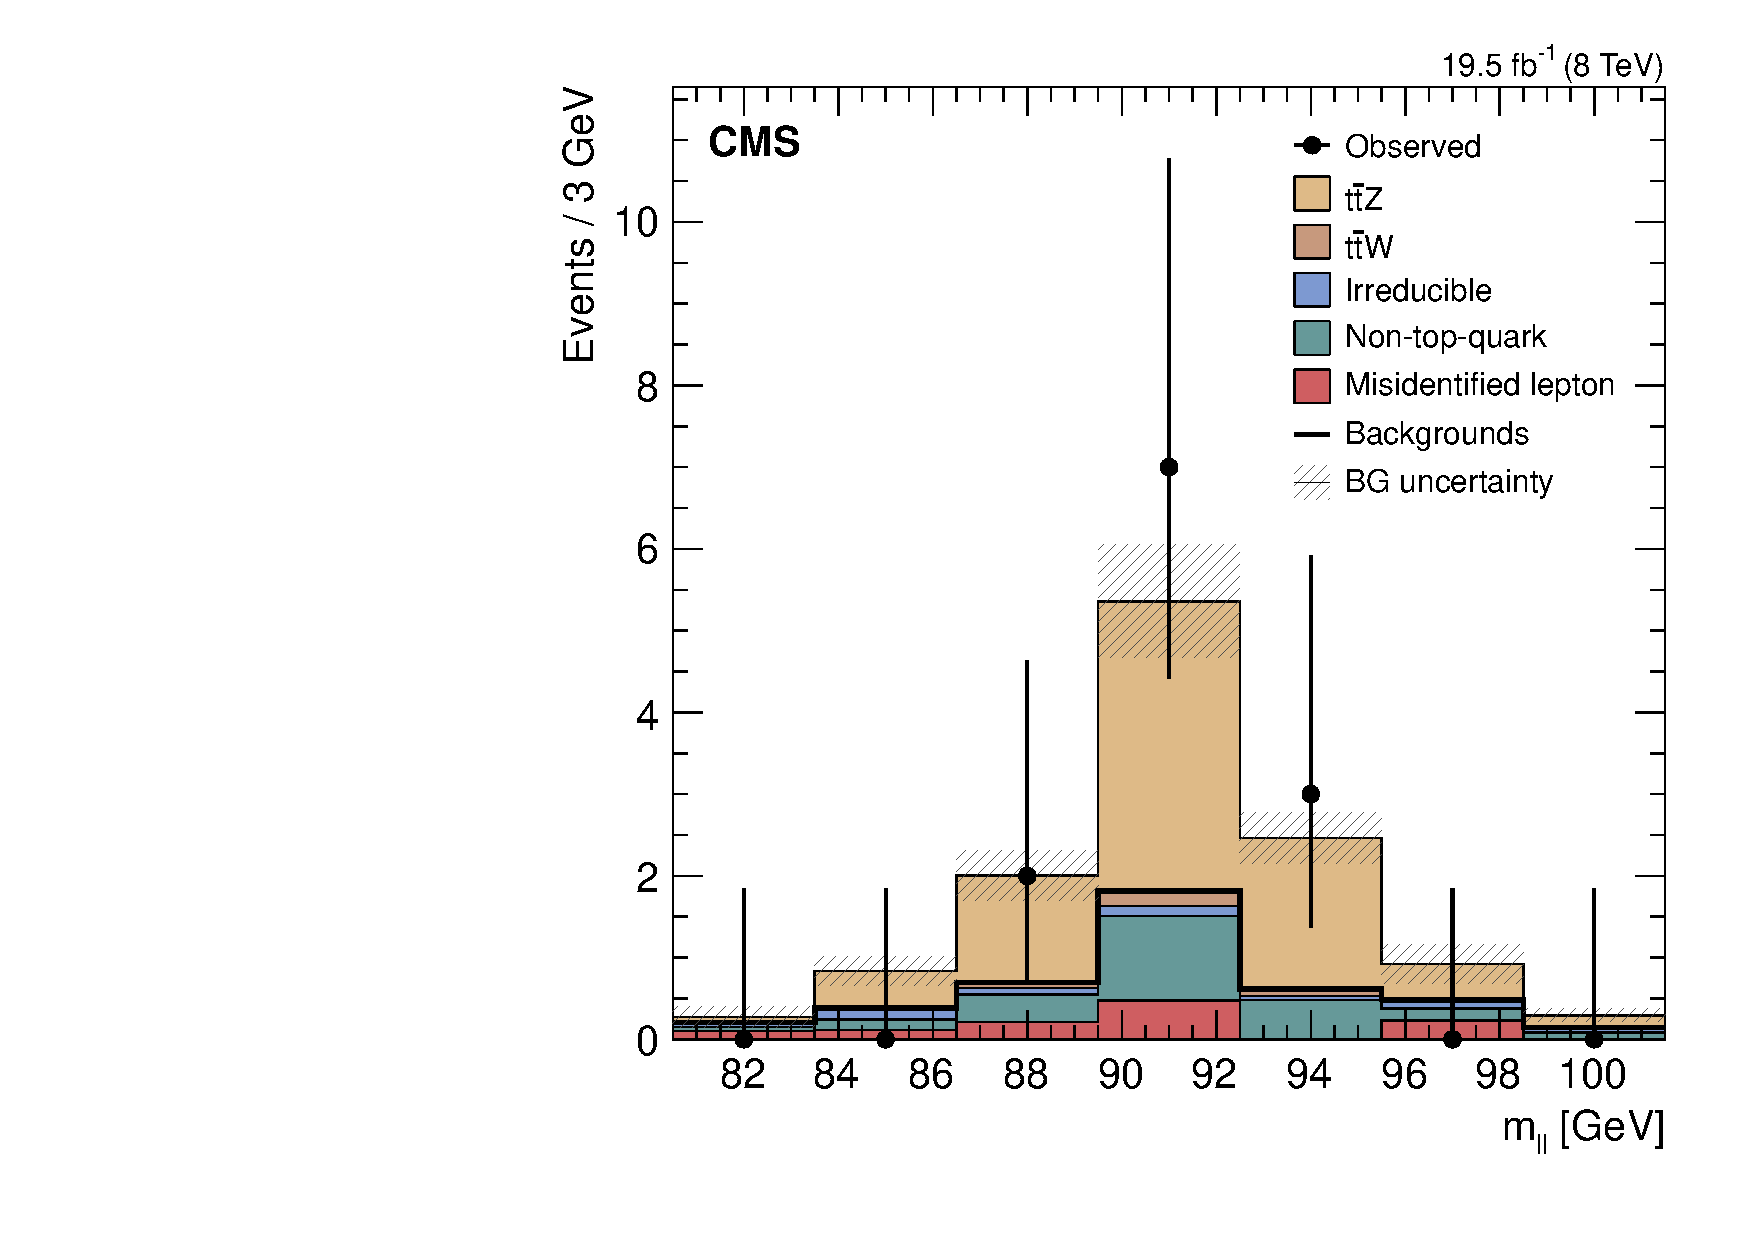
\includegraphics[width=0.48\linewidth]{Figs/Plots_Final_Selections/hZMass_3L2J2b.pdf}
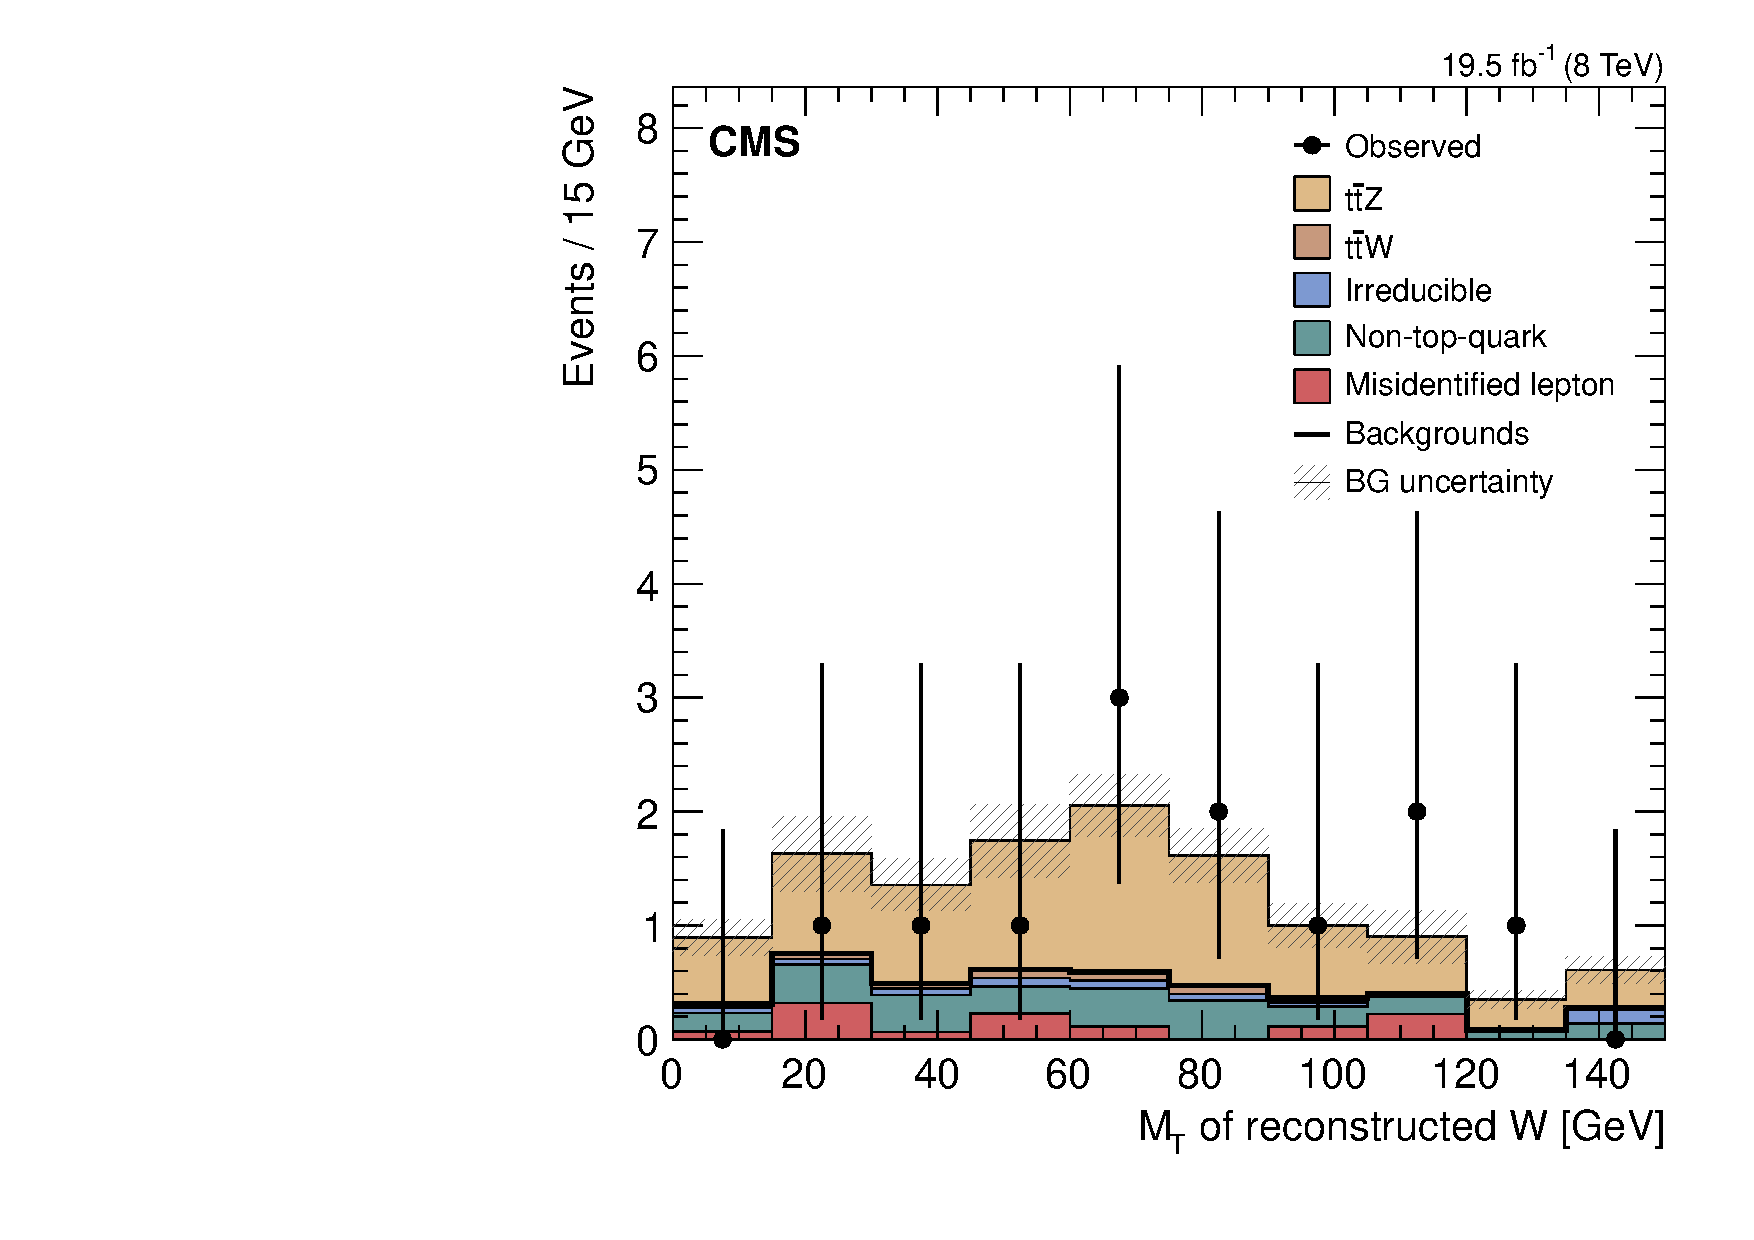
\includegraphics[width=0.48\linewidth]{Figs/Plots_Final_Selections/hWMt_3L2J2b.pdf}
\caption{\label{fig:hmass_3l2j2b}
Reconstructed mass of Z (Left) and \Mt of the W (Right) are shown after all selections have been applied.
}
\end{center}
\end{figure}


Figs~\ref{fig:hpfMET_3l2j2b} and~\ref{fig:hHt_3l2j2b} show two more defining characteristics. Both the pfMET and \HT \ are important shapes caused by the neutrino produced in the leptonic W decay and the jets produced in the top and hadronic W decay (respectively). Since these variables are not used in the current selections, they are plotted to show extra confirmation of the yields.

\begin{figure}[h]
\begin{center}
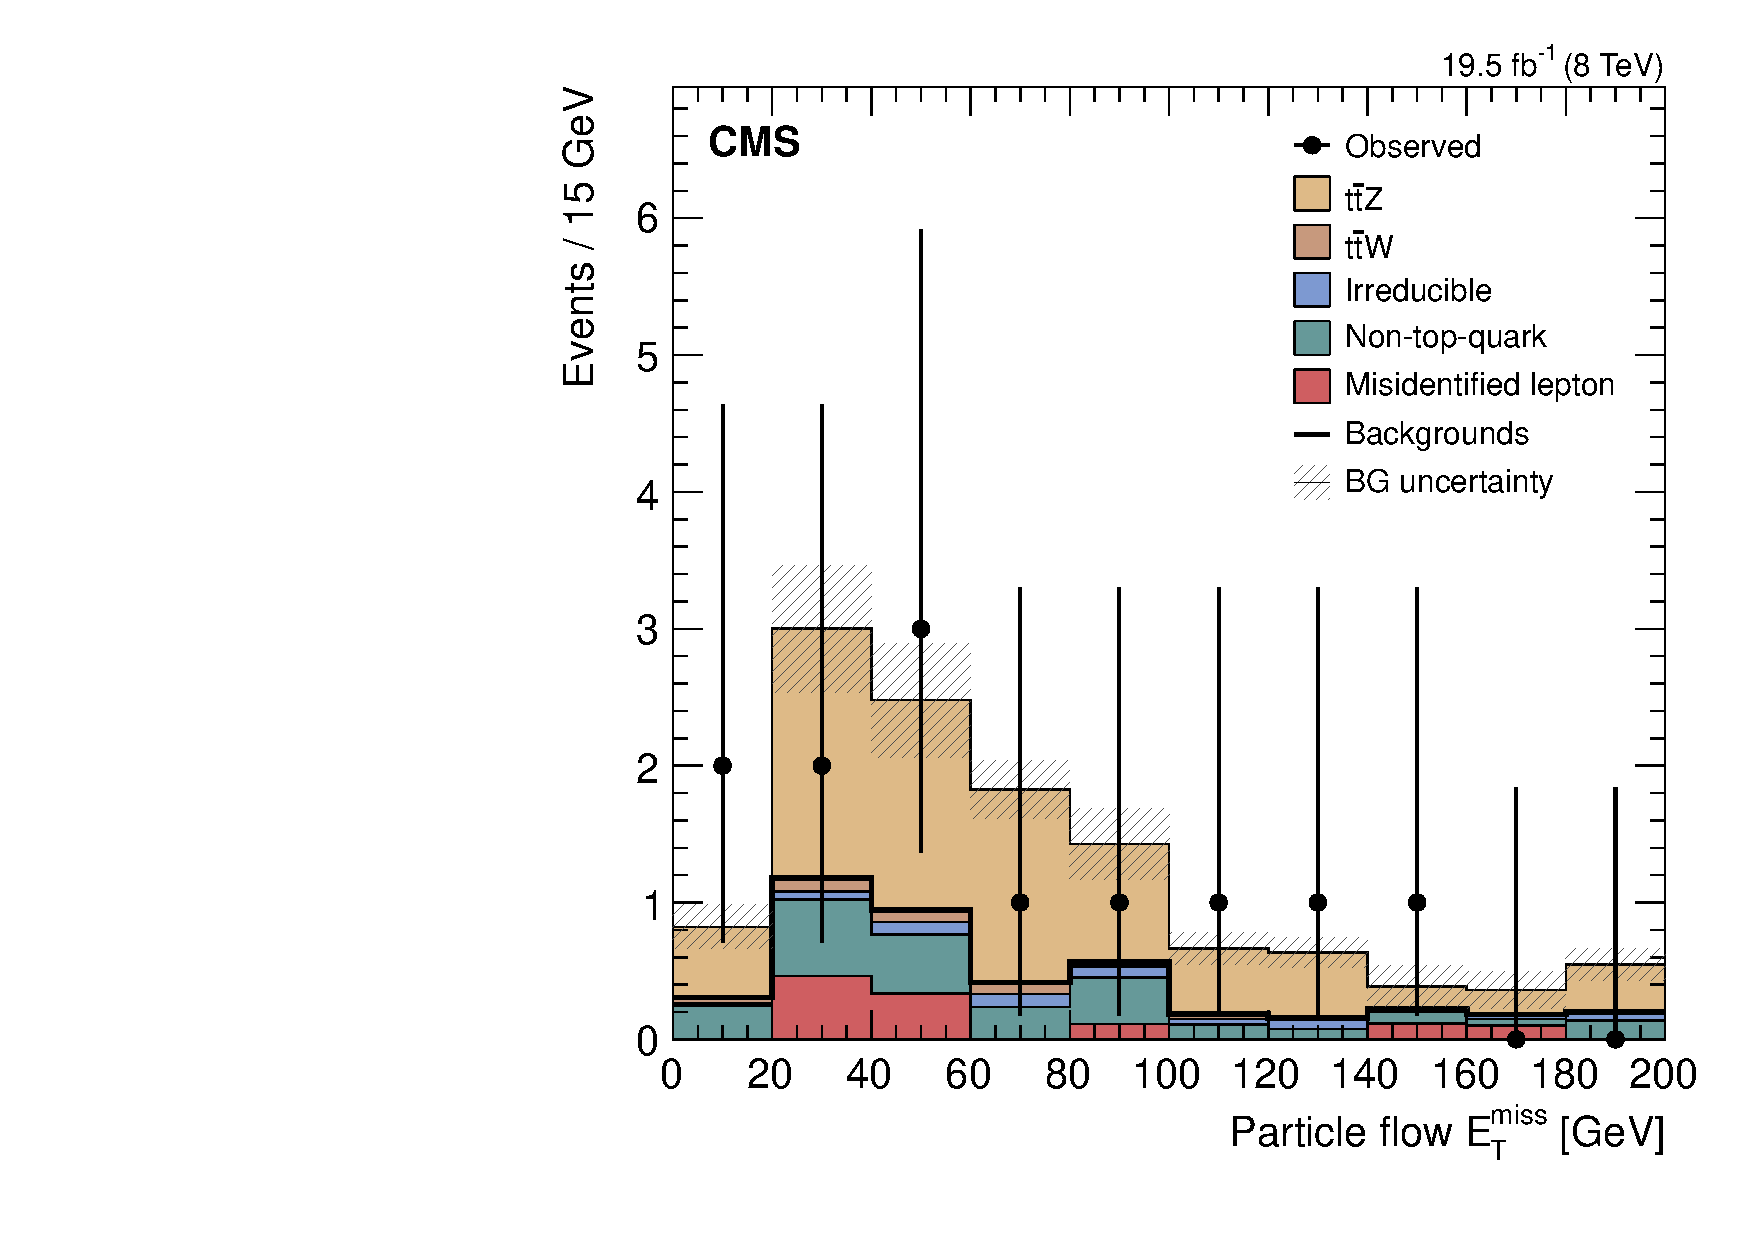
\includegraphics[width=0.48\linewidth]{Figs/Plots_Final_Selections/hpfMET_3L2J2b.pdf}
\caption{\label{fig:hpfMET_3l2j2b}
pfMET of the events after full analysis selections have been applied.
}
\end{center}
\end{figure} 

\begin{figure}[h]
\begin{center}
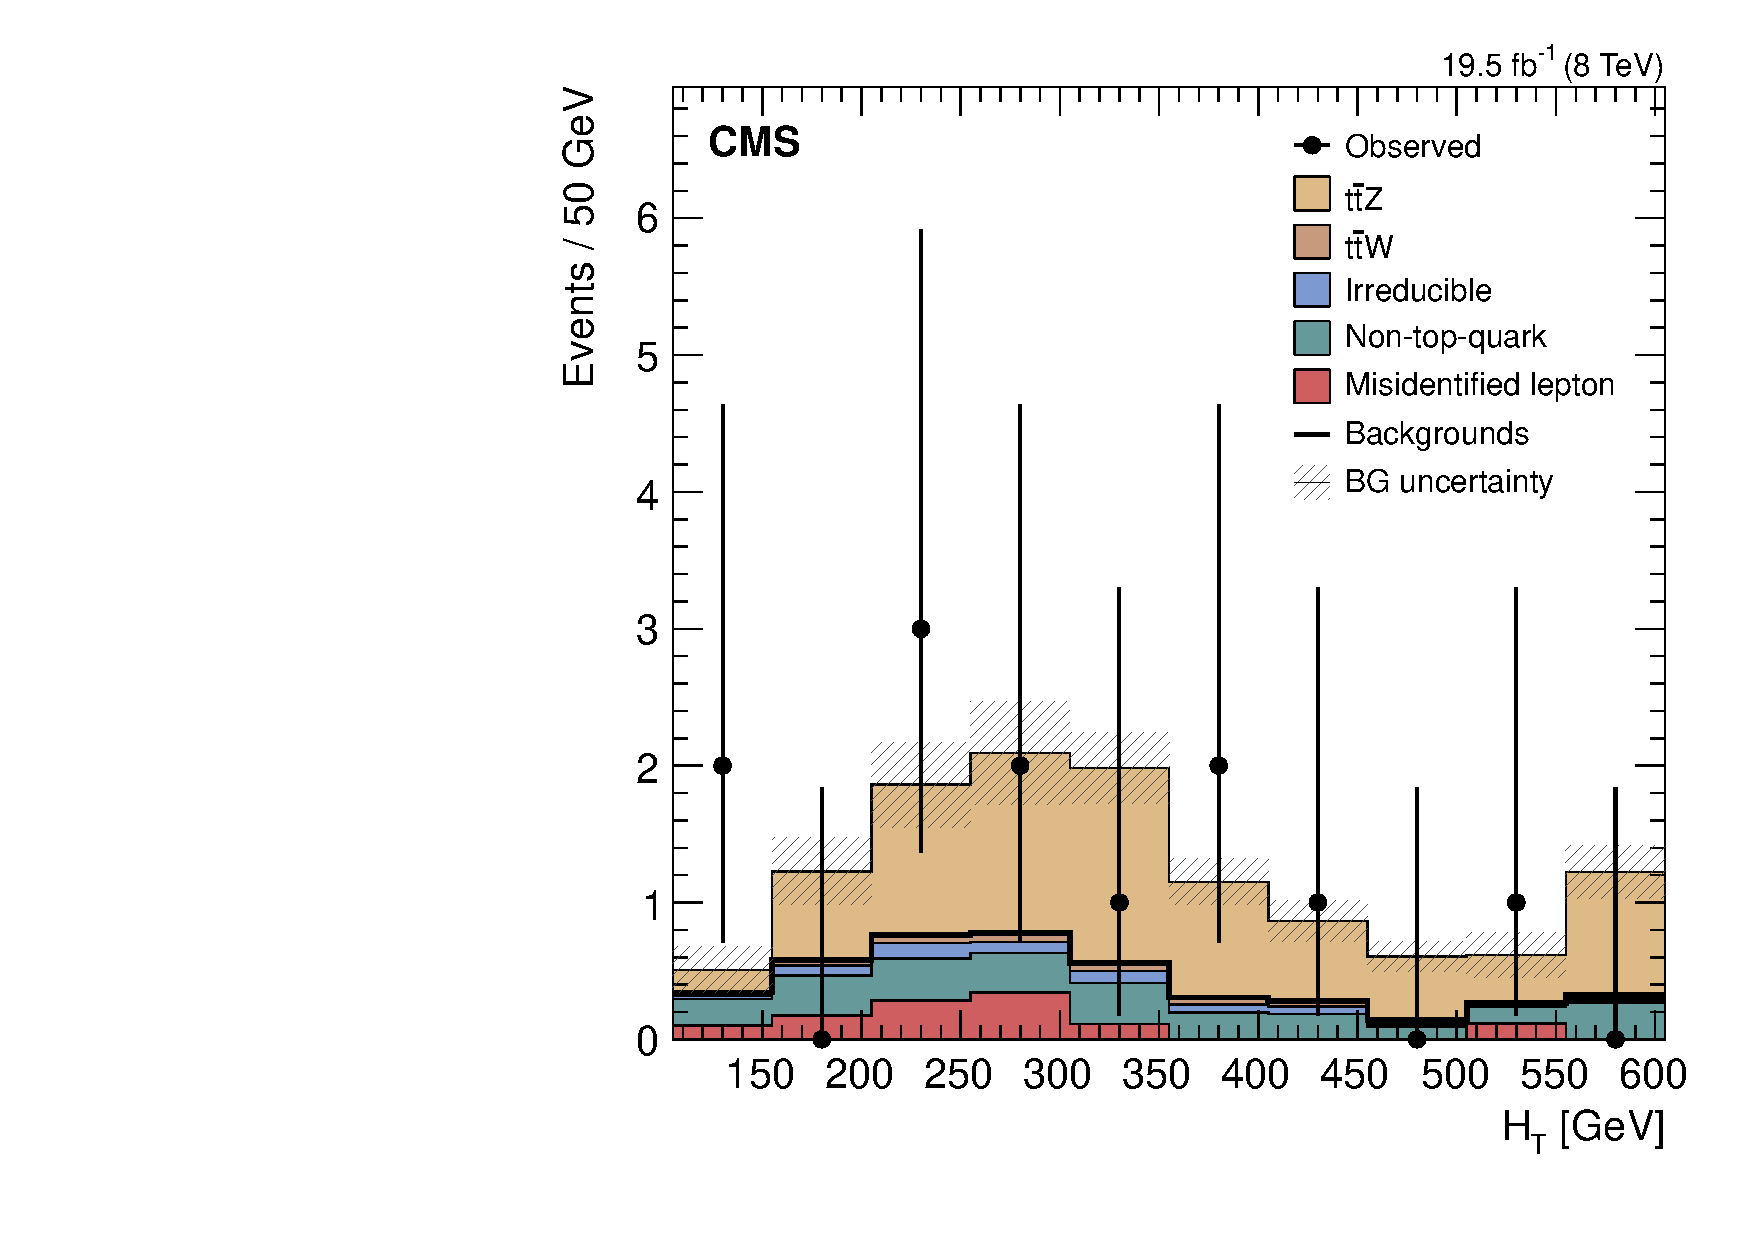
\includegraphics[width=0.48\linewidth]{Figs/Plots_Final_Selections/hHt_3L2J2b.pdf}
\caption{\label{fig:hHt_3l2j2b}
\HT \ of the events after full analysis selections have been applied.
}
\end{center}
\end{figure} 















	
	
	\section{Cross Section Calculation and Significance}
	The \ttZ \ signal is estimated in Section ~\ref{sec:signal} to be $7.62 \pm 3.46_{data\ st} \pm 0.73_{bkg\ st} \pm 1.37_{bkg\ sy}$. For the luminosity of the full dataset, we use the quoted luminosity of \intLumiwError~\cite{lumi12up}. Finally, we calculate the Branching Ratio (B) multiplied by the Acceptance of selections (A) multiplied by the Efficiency of selections ($\epsilon$) all at once. To do this, we divide the number of \ttZ \ events in MC (using the sample listed in Table ~\ref{tab:IrreducibleMCSamples}) that pass selections by the total number of \ttZ \ events in MC. This gives a BR $\times$ Acc $\times \epsilon$ of $0.0021 \pm 4.0\% _{st} \pm 10.5\% _{sy}$.\\

The full cross section is given by 
%\begin{equation}
%\begin{split}
%        %  \begin{align*}
%         \sigma &= \frac{Yields - Bkg}{\mathcal{L} \times BR \times Acc \times \epsilon}\\
%                      &=  186 \pm 85_{data\ st} \pm 18_{bkg\ st} \pm 33_{bkg\ sy} \pm 7_{BR*Acc*\epsilon\ st} \pm 20_{BR*Acc*\epsilon\ sy} \pm 5_{lumi\ sy}\ fb\\
%                      &= 186 \pm 107\ \text{fb}
%        %  \end{align*}
%        \end{split}
%\end{equation}

\begin{align}
         \sigma &= \frac{Yields - Bkg}{\mathcal{L} \times B \times A\times \epsilon}\\
                      &=  186 \pm 85_{data\ st} \pm 18_{bkg\ st} \pm 33_{bkg\ sy}\pm 7_{B*A*\epsilon\ st} \pm 20_{B*A*\epsilon\ sy} \pm 5_{lumi\ sy}\ \text{fb}\\
                      &= 186 \pm 107\ \text{fb}
\end{align}
          
          
 Additionally, the LandS software is used to perform this calculation with a bit more rigor (see~\cite{higgscomb}). Data cards are prepared from the information contained in this note. Backgrounds are assumed to be log normal with uncorrelated errors. Data driven backgrounds use the statistical and systematic uncertainties that were derived with the methods. Monte Carlo only backgrounds use the uncertainties derived in Sec~\ref{ch:eff_and_unc}. With this preparation, the signal strength (Table~\ref{tab:significance}) and ratio to theory cross section (Table~\ref{tab:landsout}) are found (where again the NLO theory cross section for \ttZ \ production is 205 fb). The final cross section measurement is $\sigma=194 _{-89} ^{+105}$ \ fb and the Ratio to Theory = $0.94 _{-0.43} ^{+0.51}$.\\
 
 
 
\begin{table}[ht!]
\begin{center}

\begin{tabular}{c|c}\hline
	& Significance	 \\ \hline
Expected	& 2.45	 \\
Measured	& 2.33	 \\
\hline
\end{tabular}
\caption{ \label{tab:significance} Expected and measured significance of the signal.}
\end{center}
\end{table}
 
\begin{table}[ht!]
\begin{center}

\begin{tabular}{c|cc}\hline
	& r        & Cross Section	 \\ \hline
	&  & \\
\ttZ	& $0.94 _{-0.43} ^{+0.51}$ & 	$194 _{-89} ^{+105}$ fb\\
& & \\
\hline
\end{tabular}
\caption{ \label{tab:landsout} Measured cross section as calculated by LandS.}
\end{center}
\end{table}
 
 
 
 
 
 
 
 \clearpage
 
 
 \section{Combined Cross Section Measurement and Significance}
 The measurement presented in this document relies on measuring the rate of production of the \ttZ process which decays into a try-lepton signature. Other final state signatures could be chosen and different techniques employed to measure the cross section of the \ttZ process in other final decay states. The advantage is that the various final states are statistically independent and thus can be combined for a reduced uncertainty on the measurement. Such a combination was performed using the results in this document as well as those determined in conjunction with Rutgers University and ETH Zurich. The combination is described in~\cite{ttV_combination}. In this combination, the cross section for the production of \ttbar~V is measured as well where V stands for both W and Z bosons. This makes the measurement a generate production of \ttbar in association with vector bosons.\\
 
 The \ttW was measured in several two lepton channels in order to maximize significance from the charge imbalance of the production. \ttZ to four leptons is measured in more than one channel to also maximize the contribution of more significant regions. This produces 9 channels in total.
 
 
 
 To maximize the sensitivity, the nine \ttW and \ttZ channels are combined. A profile likelihood scan is used to evaluate the cross-section central values and corresponding uncertainties. The same statistical procedure used in the discovery of the Higgs boson and combination of the various channels to measure the Higgs was used and 
is described in detail in Ref~\cite{higgscomb}. Table~\ref{tab:combination} summarizes the independent measurements of the various channels.

\begin{table}[!h]
%\tiny
\begin{center}
\caption{\label{tab:combination} Results of the extraction of cross sections, from single and combined channels. 
                                 The significance is expressed in terms of standard deviations.}
\begin{tabular}{c|c|c|c}
\hline
\hline
Channels used & Process &  Cross section & Significance  \\
\hline


2$\ell$ &  \ttW & $170 ^{+90}_{-80} \textrm{(stat.)} ^{+70}_{-70} \textrm{(syst.)}$  fb & 1.6 \\
3$\ell$+4$\ell$ &  \ttZ & $200 ^{+80}_{-70} \textrm{(stat.)} ^{+40}_{-30} \textrm{(syst.)}$ fb & 3.1 \\
2$\ell$+3$\ell$+4$\ell$ & \ttW $+$ \ttZ & $380 ^{+100}_{-90} \textrm{(stat.)} ^{+80}_{-70} \textrm{(syst.)}$ fb & 3.7 \\
%2L+3L+4L & $180 ^{+175}_{-168} \textrm{(total)}$ fb & --- & $218 ^{+159}_{-118} \textrm{(total)}$  fb & --- & --- & --- \\
\hline
\hline
\end{tabular}
\end{center}
\end{table}

\begin{table}[!h]
%\tiny
\begin{center}
\caption{\label{tab:fit2d} Results for the two dimensional fit of the \ttW and \ttZ cross sections.}
\begin{tabular}{c|c|c}
\hline
\hline
Channels used & \ttW  cross section &  \ttZ{} cross section \\
\hline

2$\ell$+3$\ell$+4$\ell$ & $170 ^{+110}_{-100} \textrm{(total)}$ fb & $200 ^{+90}_{-90} \textrm{(total)}$ fb  \\

\hline
\hline
\end{tabular}
\end{center}
\end{table}



In order to combine the \ttZ channels, a one-dimensional fit is performed on all of the channels. A one-dimensional fit is also performed on the \ttW channels. This fit maximizes the contributions from the most significant channels. From the same-sign dilepton channels, the extracted \ttW cross section is measured to be  $170 ^{+90}_{-80} \textrm{(stat.)} ^{+70}_{-70} \textrm{(syst.)}$~fb, with a significance of $1.6$ standard deviations. The three and four lepton channels combined to a measured \ttZ cross section of 
$200 ^{+80}_{-70} \textrm{(stat.)} ^{+40}_{-30} \textrm{(syst.)}$~fb, with a significance of $3.1$ standard deviations. 

Because each measurement depends on the value of the other process (e.g. \ttZ relies on the \ttW cross section in it's measurement), the cross section of the second process is constrained to the theoretical SM value with a systematic uncertainty of 50\%.

To gauge the impact of using the constrained value, it is varied. The measured \ttW cross section varies by approximately 10\% 
when the theoretical \ttZ cross section is altered up to 1.5 times its nominal theoretical value.  
Performing the same procedure with the \ttW theoretical value, the variation of the measured \ttZ cross section 
is less than 2\%. 

\begin{figure}[!h]
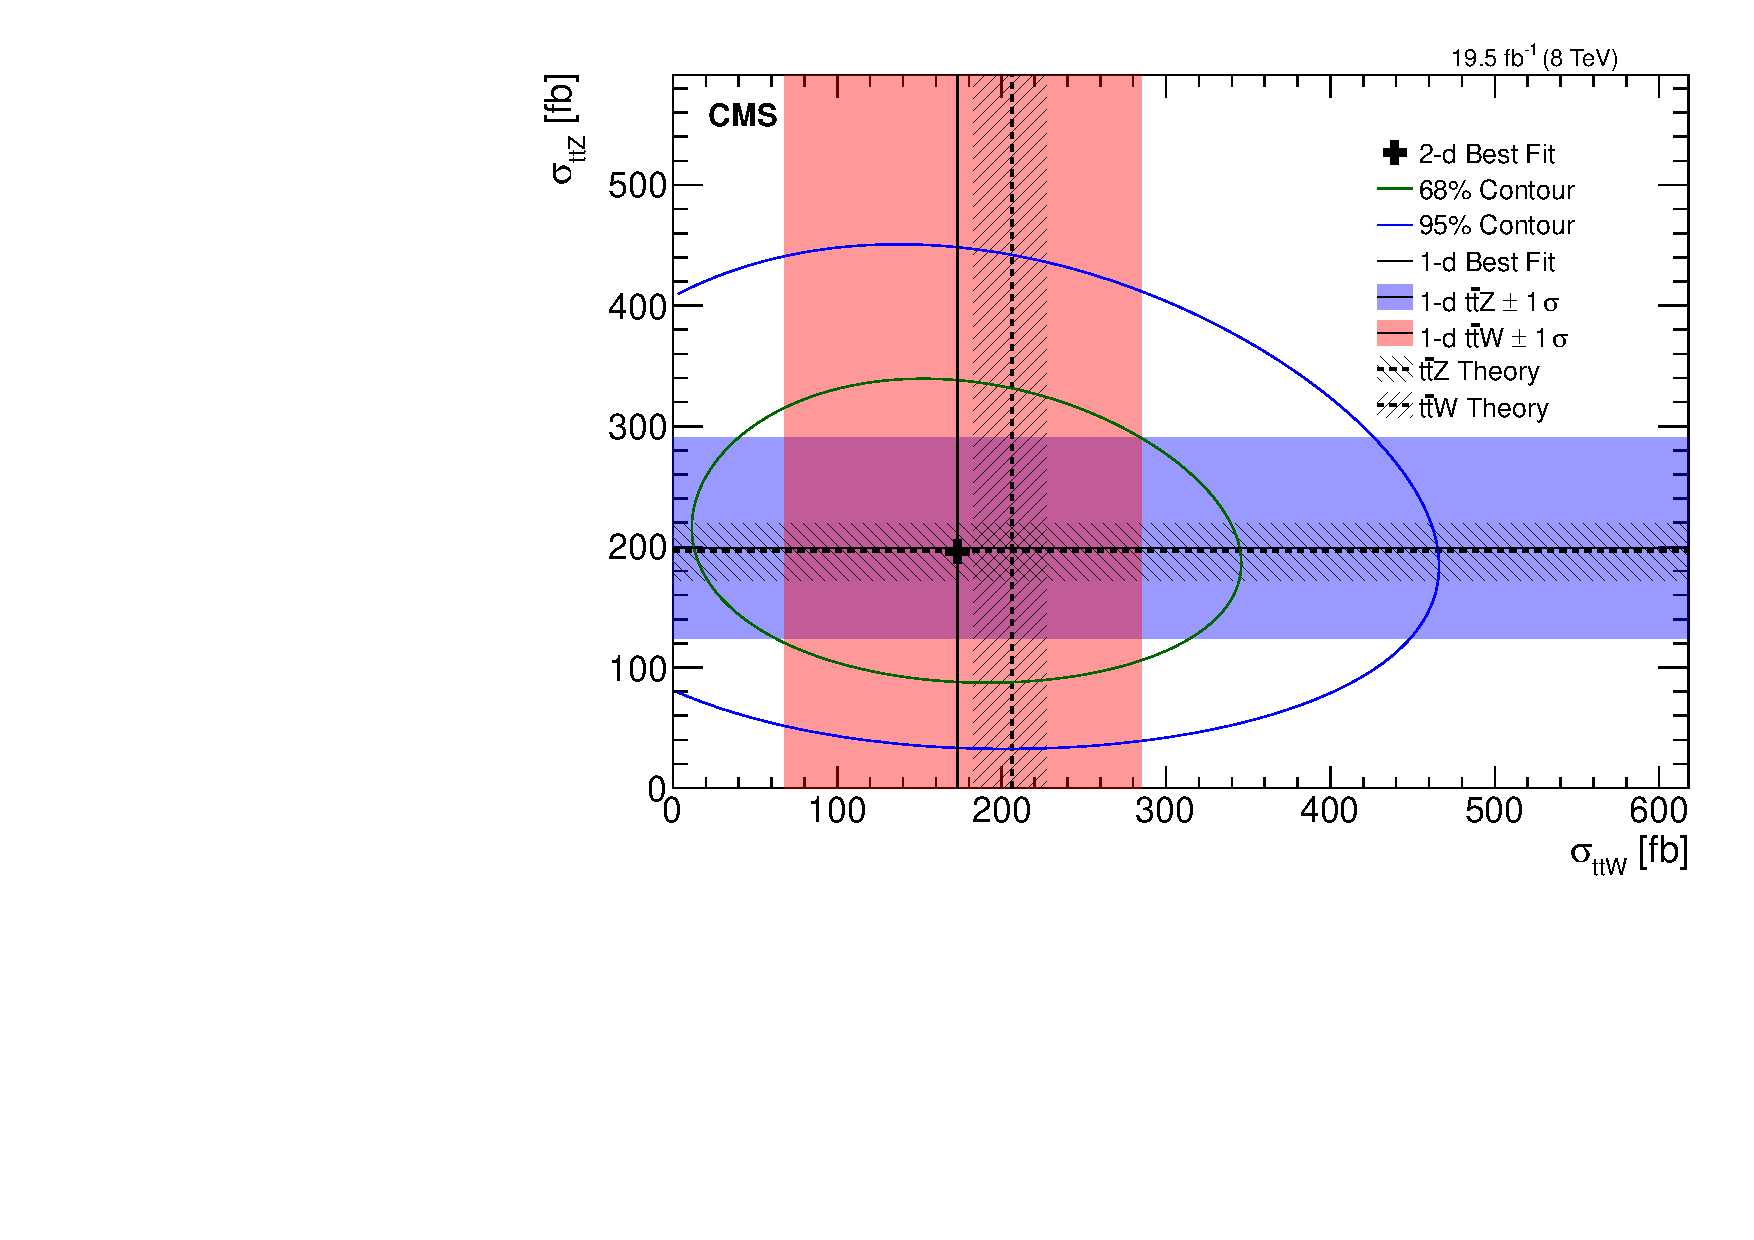
\includegraphics[width=0.8\linewidth]{fit_2d.pdf}
\caption{\label{fig:combination_2d} The result of the two-dimensional best fit for \ttW and \ttZ{} cross sections 
%($\textbf{+}$ symbol) 
(cross symbol) 
is shown along with its 68 and 95\% confidence level contours. The result of this fit is superimposed with the 
separate \ttW and \ttZ{} cross section measurements, and the corresponding 1$\sigma$ bands, obtained 
from the dilepton, and the trilepton/four-lepton channels, respectively. The figure also shows the 
predictions from theory and the corresponding uncertainties.}
\end{figure}

A more sophisticated approach can be taken to allow both measurements to feed back into each other and remove the reliance on the theoretical cross sections. A simultaneous fit is performed on the two processes using all of the channels. The two-dimensional fit is represented graphically in Fig~\ref{fig:combination_2d} and Table~\ref{tab:fit2d} summarizes the cross sections numerically. Within uncertainties the 2 one-dimensional fits and the 1 two-dimensional fit produce the same measurement for the \ttZ and \ttW cross sections.



%
Finally, a one-dimensional fit of all channels is performed to extract a combined cross section 
$\sigma_{\ttbar\textrm{V}} = 380 ^{+100}_{-90} \textrm{(stat.)} ^{+80}_{-70} \textrm{(syst.)}$~fb 
%, where V stands for W or Z, 
with a significance of 3.7 standard deviations. 
%

 
	
